%%%%%%%%%%%%%%%%%%%%%%%%%%%%%%%%%%%%
%% 
%% Renaissance and Reformation
%% 
%% Key Events:
%% 
%% 
%% Key Ideas:
%% 
%% 
%% Style: 
%% 
%% Figures:
%% A/M/L:
%% R/P/P:
%% 
%%%%%%%%%%%%%%%%%%%%%%%%%%%%%%%%%%%%

\firstslide[29 May 2012]{Renaissance and Reformation}

\section{Renaissance in the South}

\subsection{Changing Beliefs}
\begin{frame}{Changing Beliefs}
	\begin{itemize}
		\item<1->Medieval cosmology: concentric circles and geocentrism.
		\item<2->Dante's \emph{Divine Comedy} (1308--1321).
			\only<3-5>{
			\begin{itemize}
				\item<3-5>Inferno
					\only<3>{
						\begin{enumerate}
							\item Vestibule
							\item Limbo
							\item Lust
							\item Gluttony
							\item Greed
							\item Anger
							\item Heresy
							\item Violence
							\item Fraud
							\item Treachery
						\end{enumerate}
					}
				\item<4-5>Purgatory
					\only<4>{
						\begin{enumerate}
							\item Ante-Purgatory (1): Excommunicate
							\item Ante-Purgatory (2): Late Repentant
							\item The proud
							\item The envious
							\item The wrathful
							\item The slothful
							\item The covetous
							\item The gluttonous
							\item The lustful
							\item The earthly paradise
						\end{enumerate}
					}
				\item<5-5>Paradise
					\only<5>{
						\begin{enumerate}
							\item The Moon: The Inconstant
							\item Mercury: The Ambitious
							\item Venus: The Lovers
							\item The Sun: The Wise
							\item Mars: The Warriors of the Faith
							\item Jupiter: The Just Rulers
							\item Saturn: The Contemplatives
							\item The Fixed Stars: Faith, Hope, and Love
							\item The Primum Mobile: The Angels
							\item The Empyrean (the abode of God)
						\end{enumerate}
					}
			\end{itemize}
			}
		\item<6->Copernicus (1473--1543).
		\item<7->1492. Columbus sails the ocean blue.
	\end{itemize}
\end{frame}

\begin{frame}{Changing Beliefs}
	Columbus's Strange Idea \\
	\includegraphics[width=4in]{img/map-world-columbus.pdf}
\end{frame}

\subsection{Reformations}
\begin{frame}{From Council to Reformations}
	\begin{itemize}
		\item<1->1414--1417. Council of Constance and its question of authority.
		\item<2->1415. Jan Hus executed (indulgences).
		\item<3->Erasmus (1466--1536).
		\item<4->1480. Spanish Inquisition Established.
		\item<5->Martin Luther (1483--1546).
		\item<6->Ulrich Zwingli (1484--1531) in Z{\"u}rich.
		\item<7->John Calvin (1509--1564) in Geneva.
		\item<8->1534. Henry VIII establishes Church of England.
		\item<9->1552. Counter-Reformation: Council of Trent (1545--1564).
		\item<10->1555. Peace of Augsburg.
	\end{itemize}
\end{frame}

\subsection{Art}
\begin{frame}{Art}
	\only<1>{
		\begin{center}
			Florence \\
			\includegraphics[height=3in]{img/map-italy.pdf}
		\end{center}
	}
	\only<2>{
		\begin{center}
			Major Artists
		\end{center}

		\begin{itemize}
			\item Sandro Botticelli (Alessandro di Mariano di Vanni Filipepi) [1445--1510]
			\item Teenage Mutant Ninja Turtles (not really)
			\begin{enumerate}
				\item Donatello (Donato di Niccolò di Betto Bardi) [1386--1466]
				\item Leonardo (da Vinci) [1452--1519]
				\item Michelangelo (di Lodovico Buonarroti Simoni) [1475--1564]
				\item Raphael (Raffaello Sanzio da Urbino) [1483--1520]
			\end{enumerate}
			\item (Michelangelo Merisi da) Caravaggio [1571--1610]
		\end{itemize}
	}
	\only<3>{
		Botticelli's \emph{Birth of Venus} [1486] (again)
 		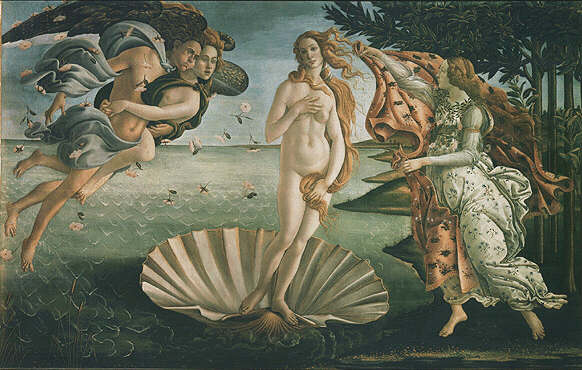
\includegraphics[width=4in]{img/img-venus.jpeg}
	}
	\only<4>{
		Da Vinci's \emph{The Last Supper} [1498]
		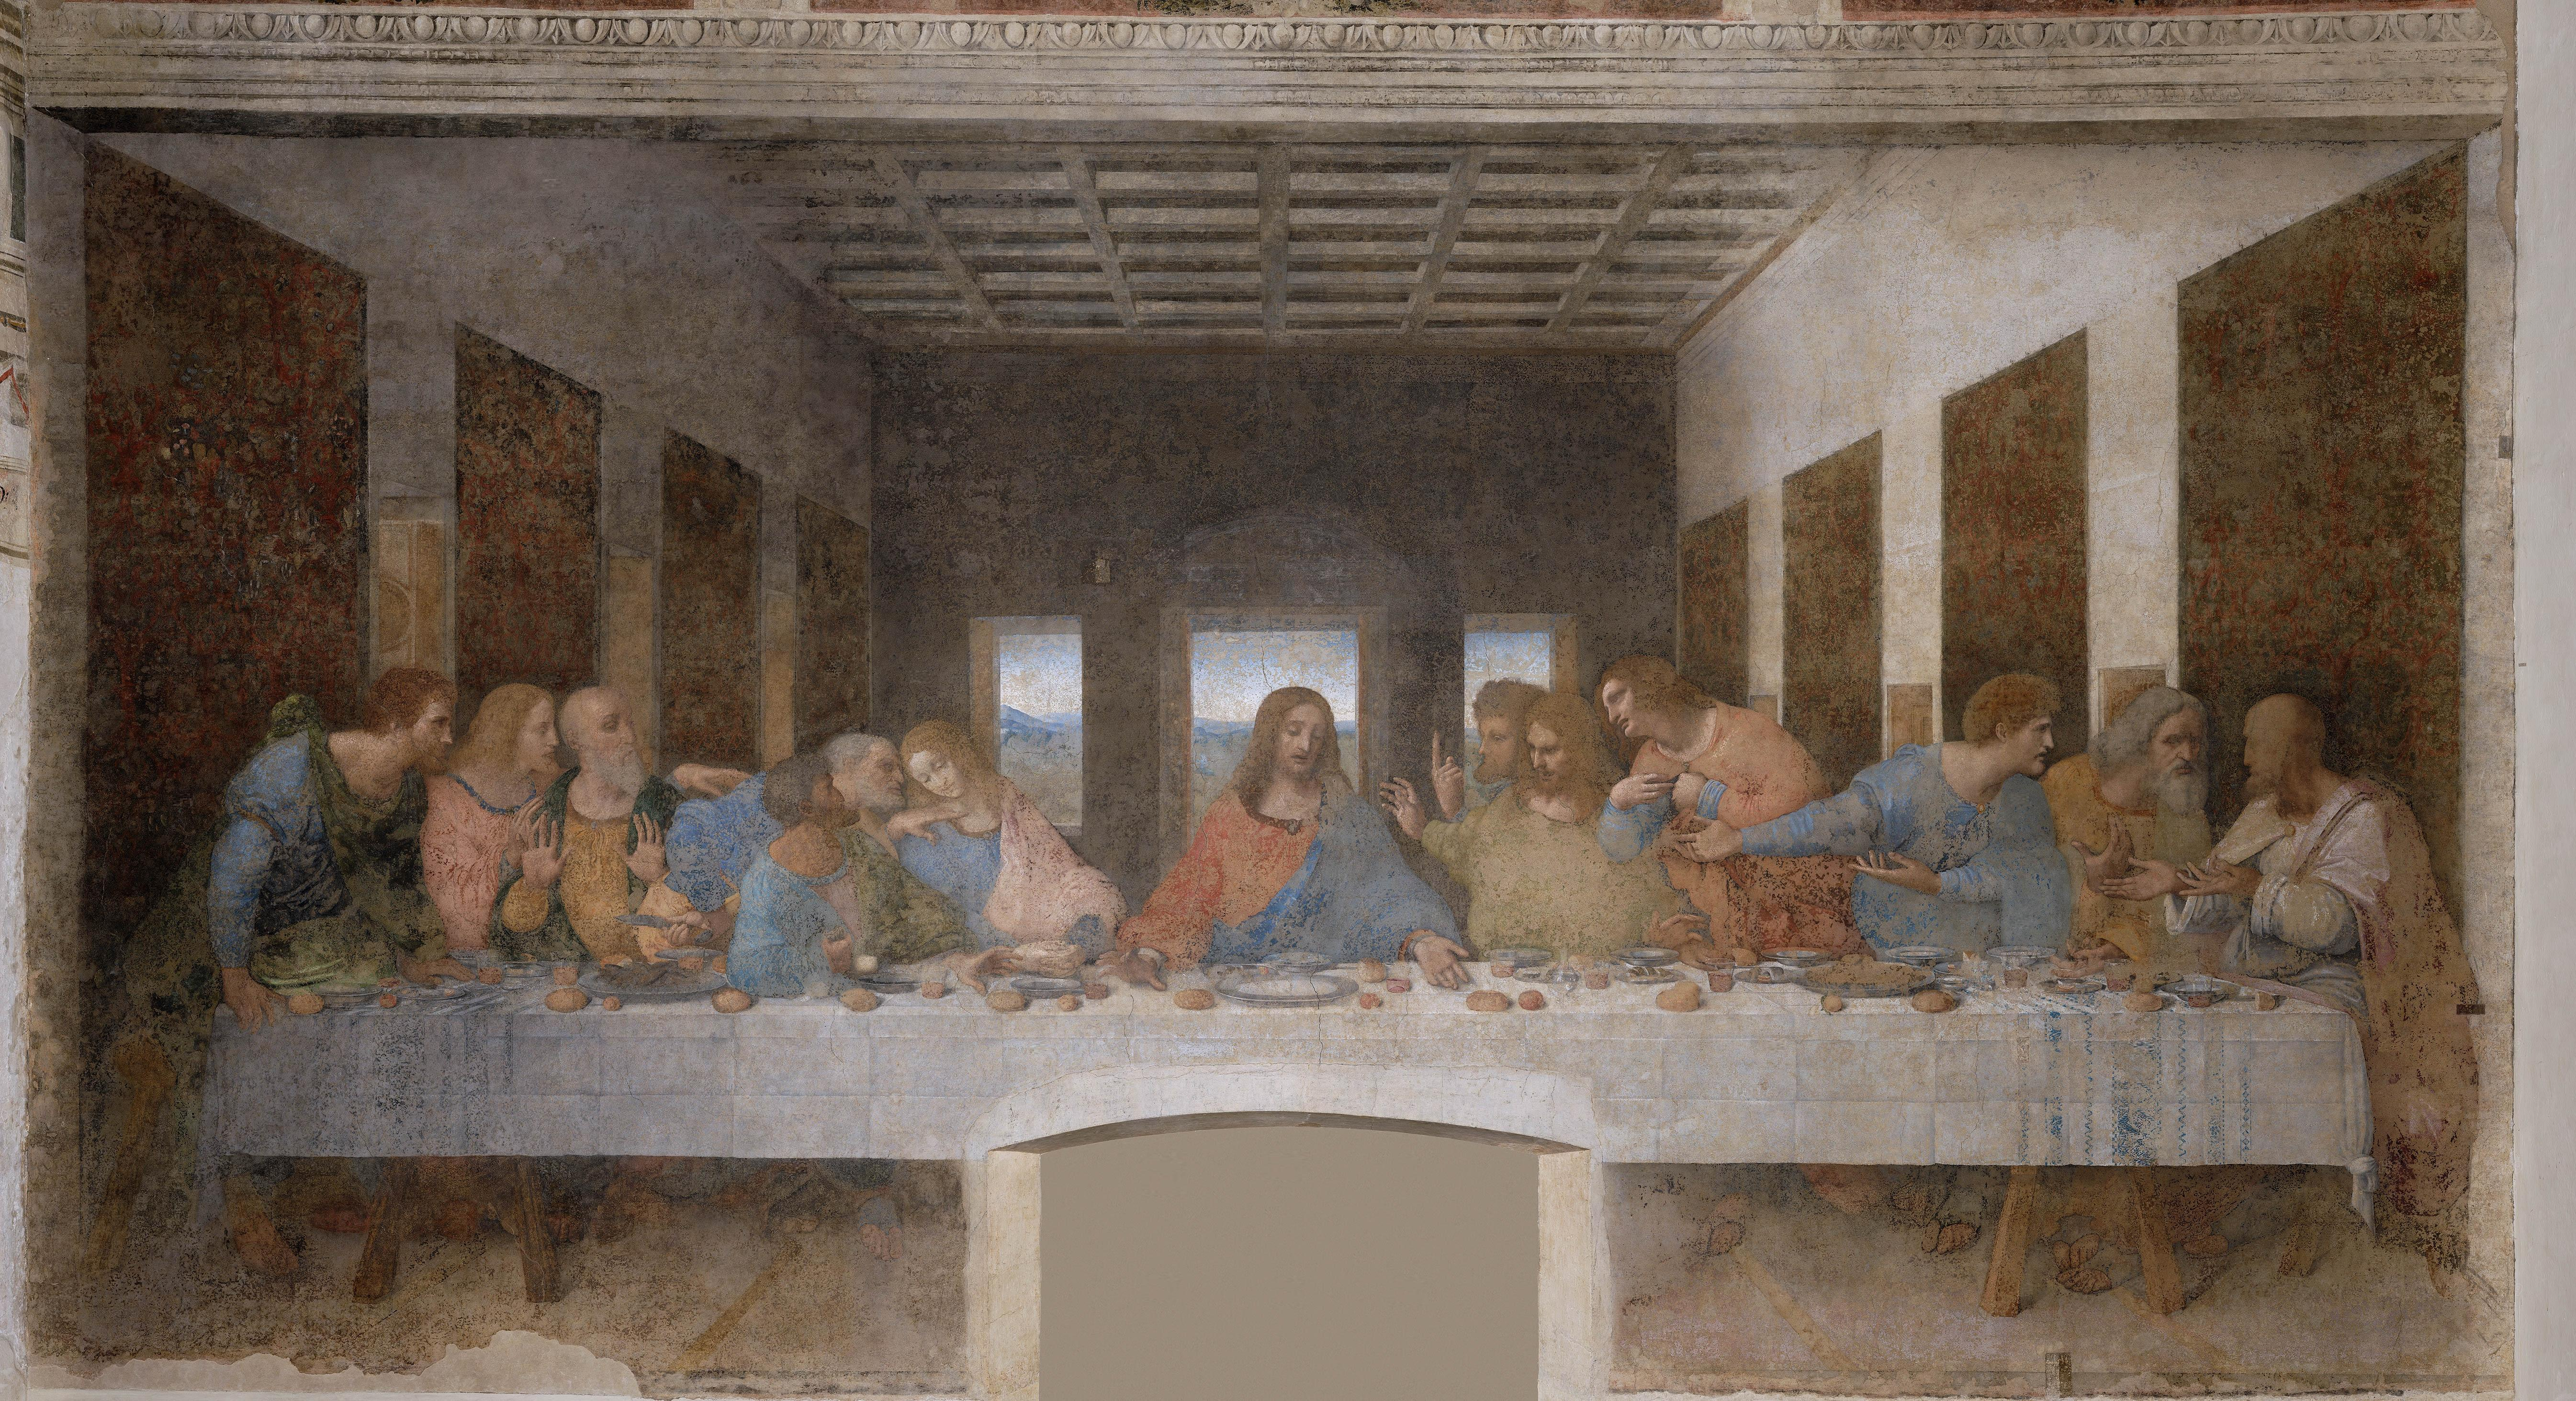
\includegraphics[width=4in]{img/img-supper.jpeg}
	}
	\only<5>{
		Da Vinci's \emph{Mona Lisa} [1503--1507]
		\begin{center}
			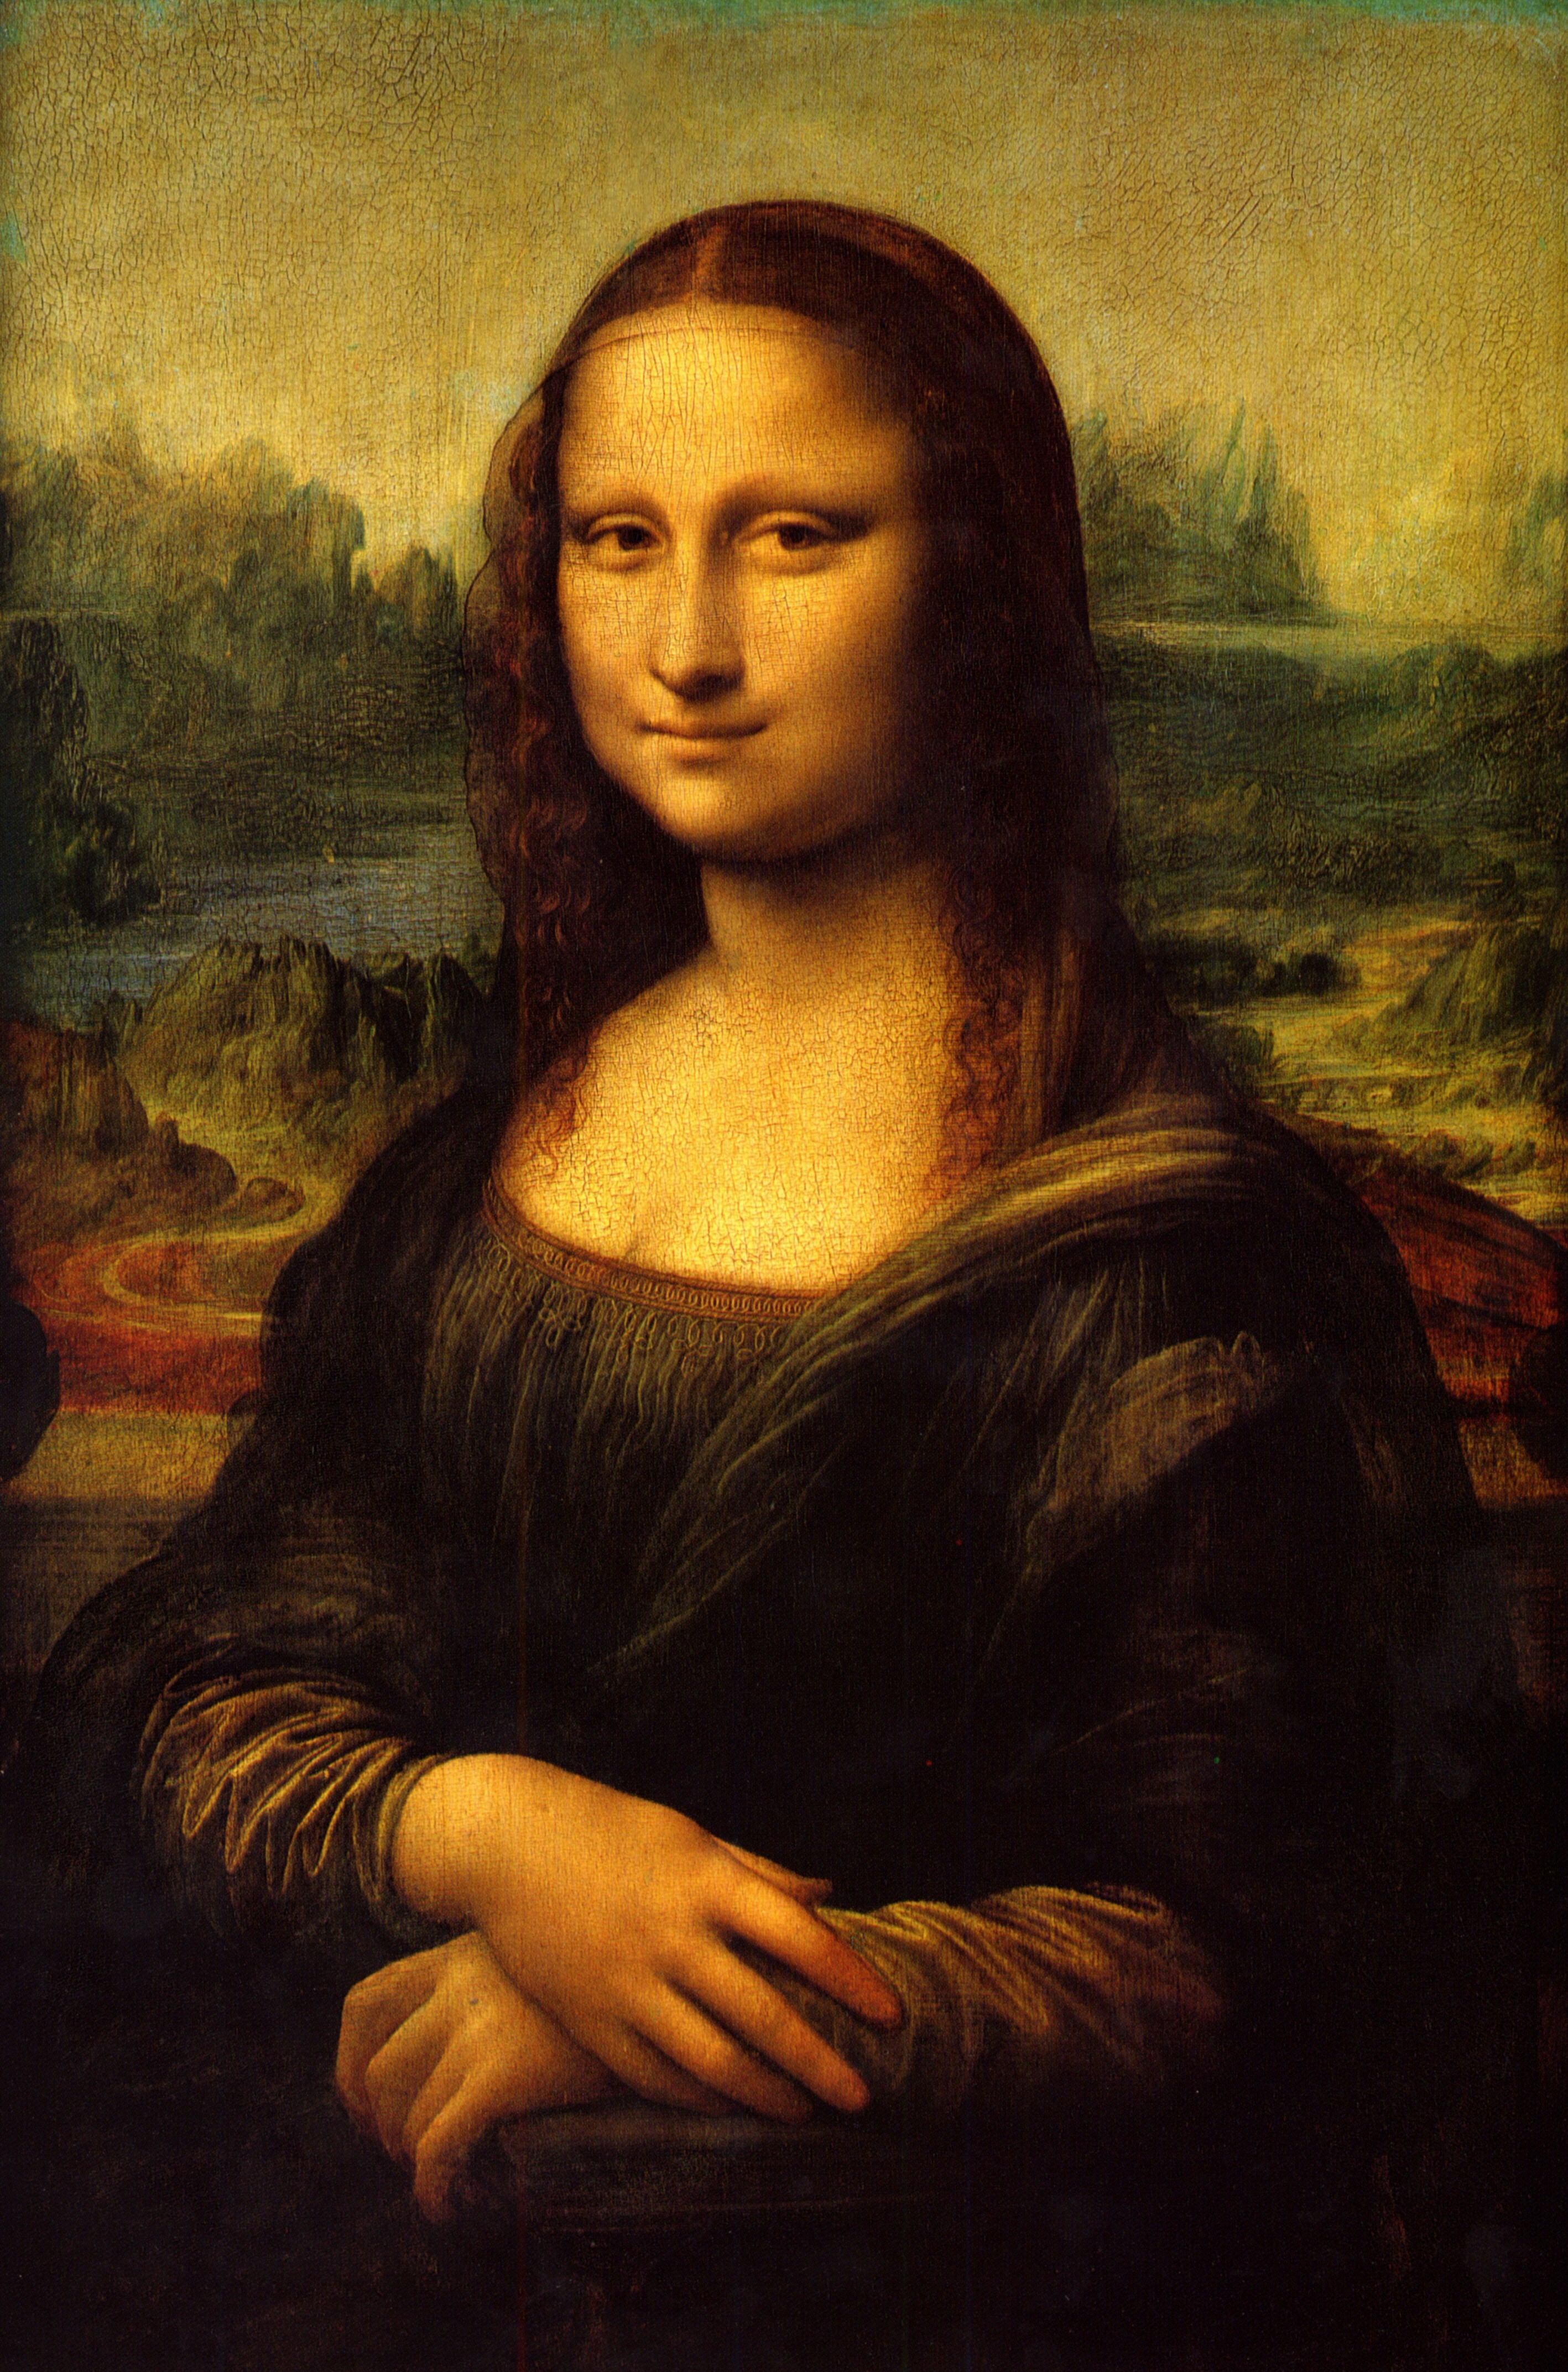
\includegraphics[height=2.9in]{img/img-lisa.jpeg}
		\end{center}
	}
	\only<6>{
		Michelangelo's \emph{David} [1504]
		\begin{center}
			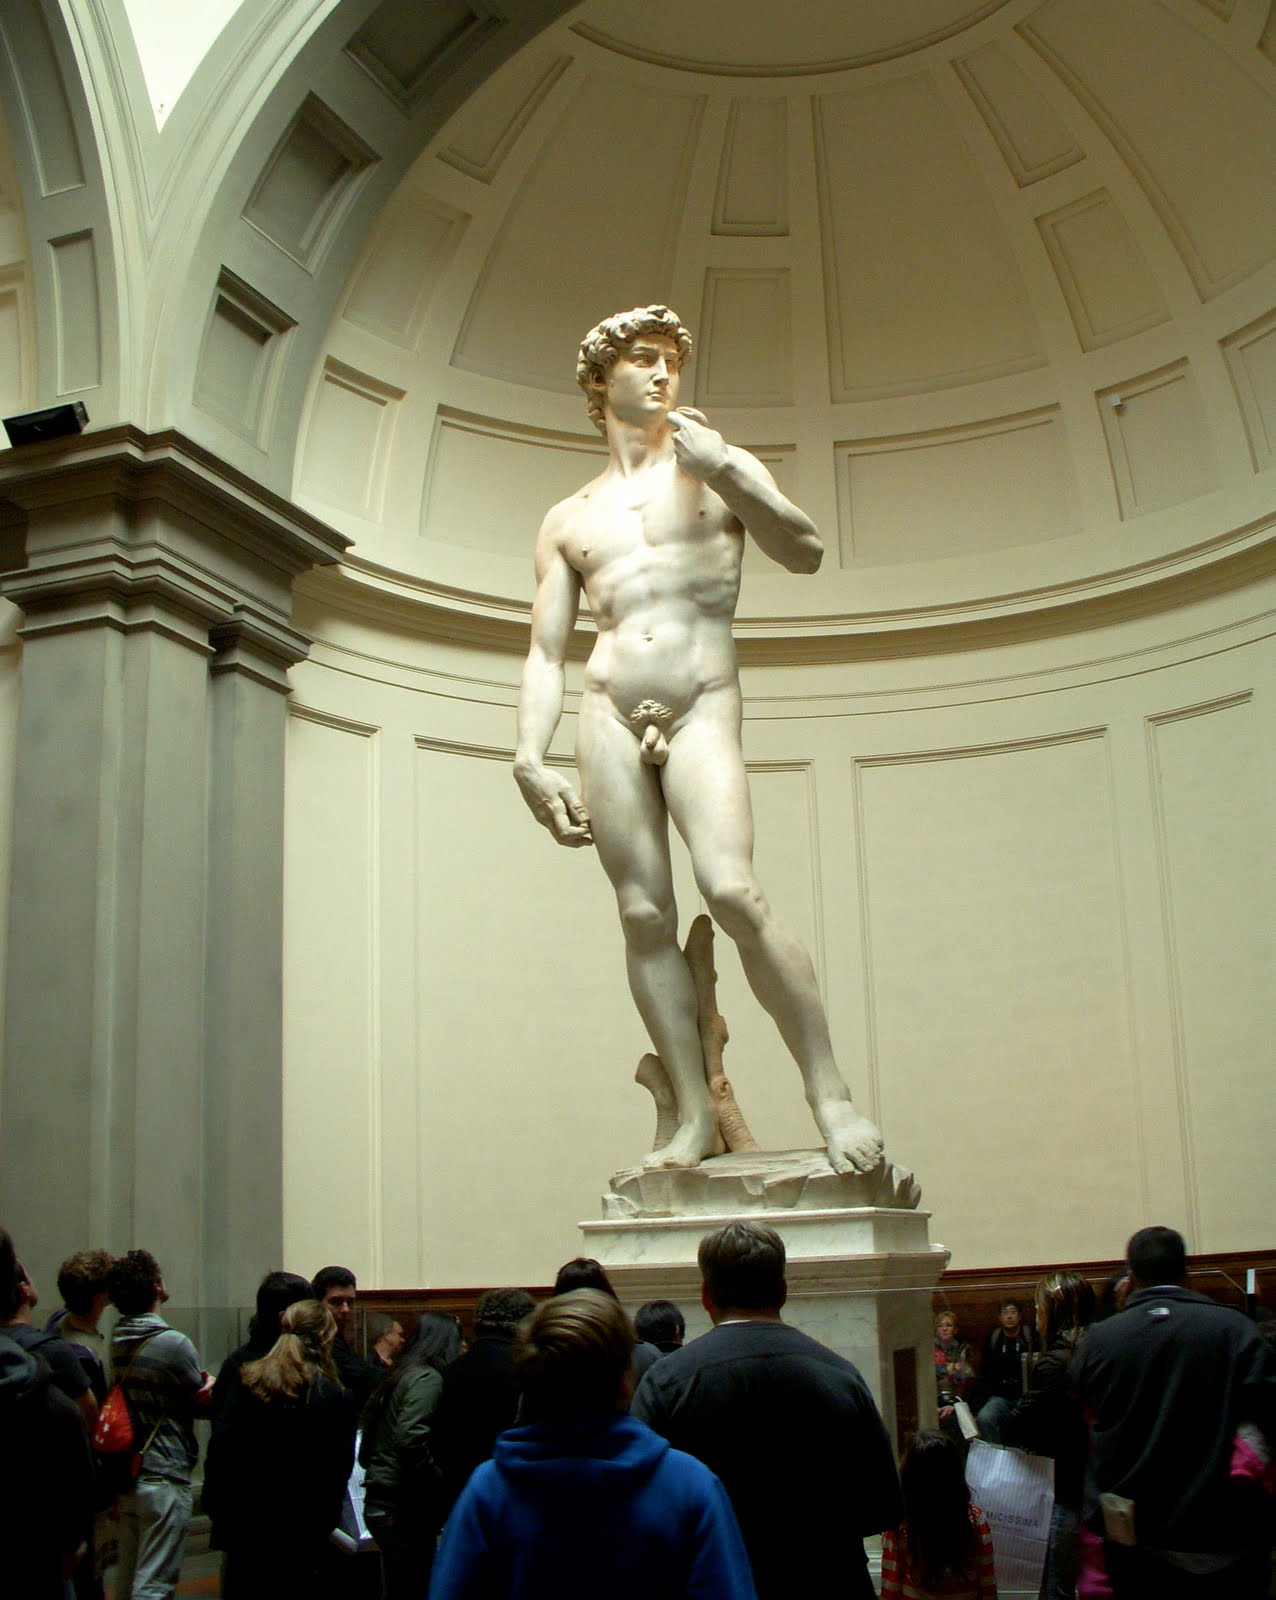
\includegraphics[height=2.8in]{img/img-david.jpeg}
		\end{center}

	}
	\only<7>{
		Michelangelo's \emph{Sistine Chapel} [1508--1512]
		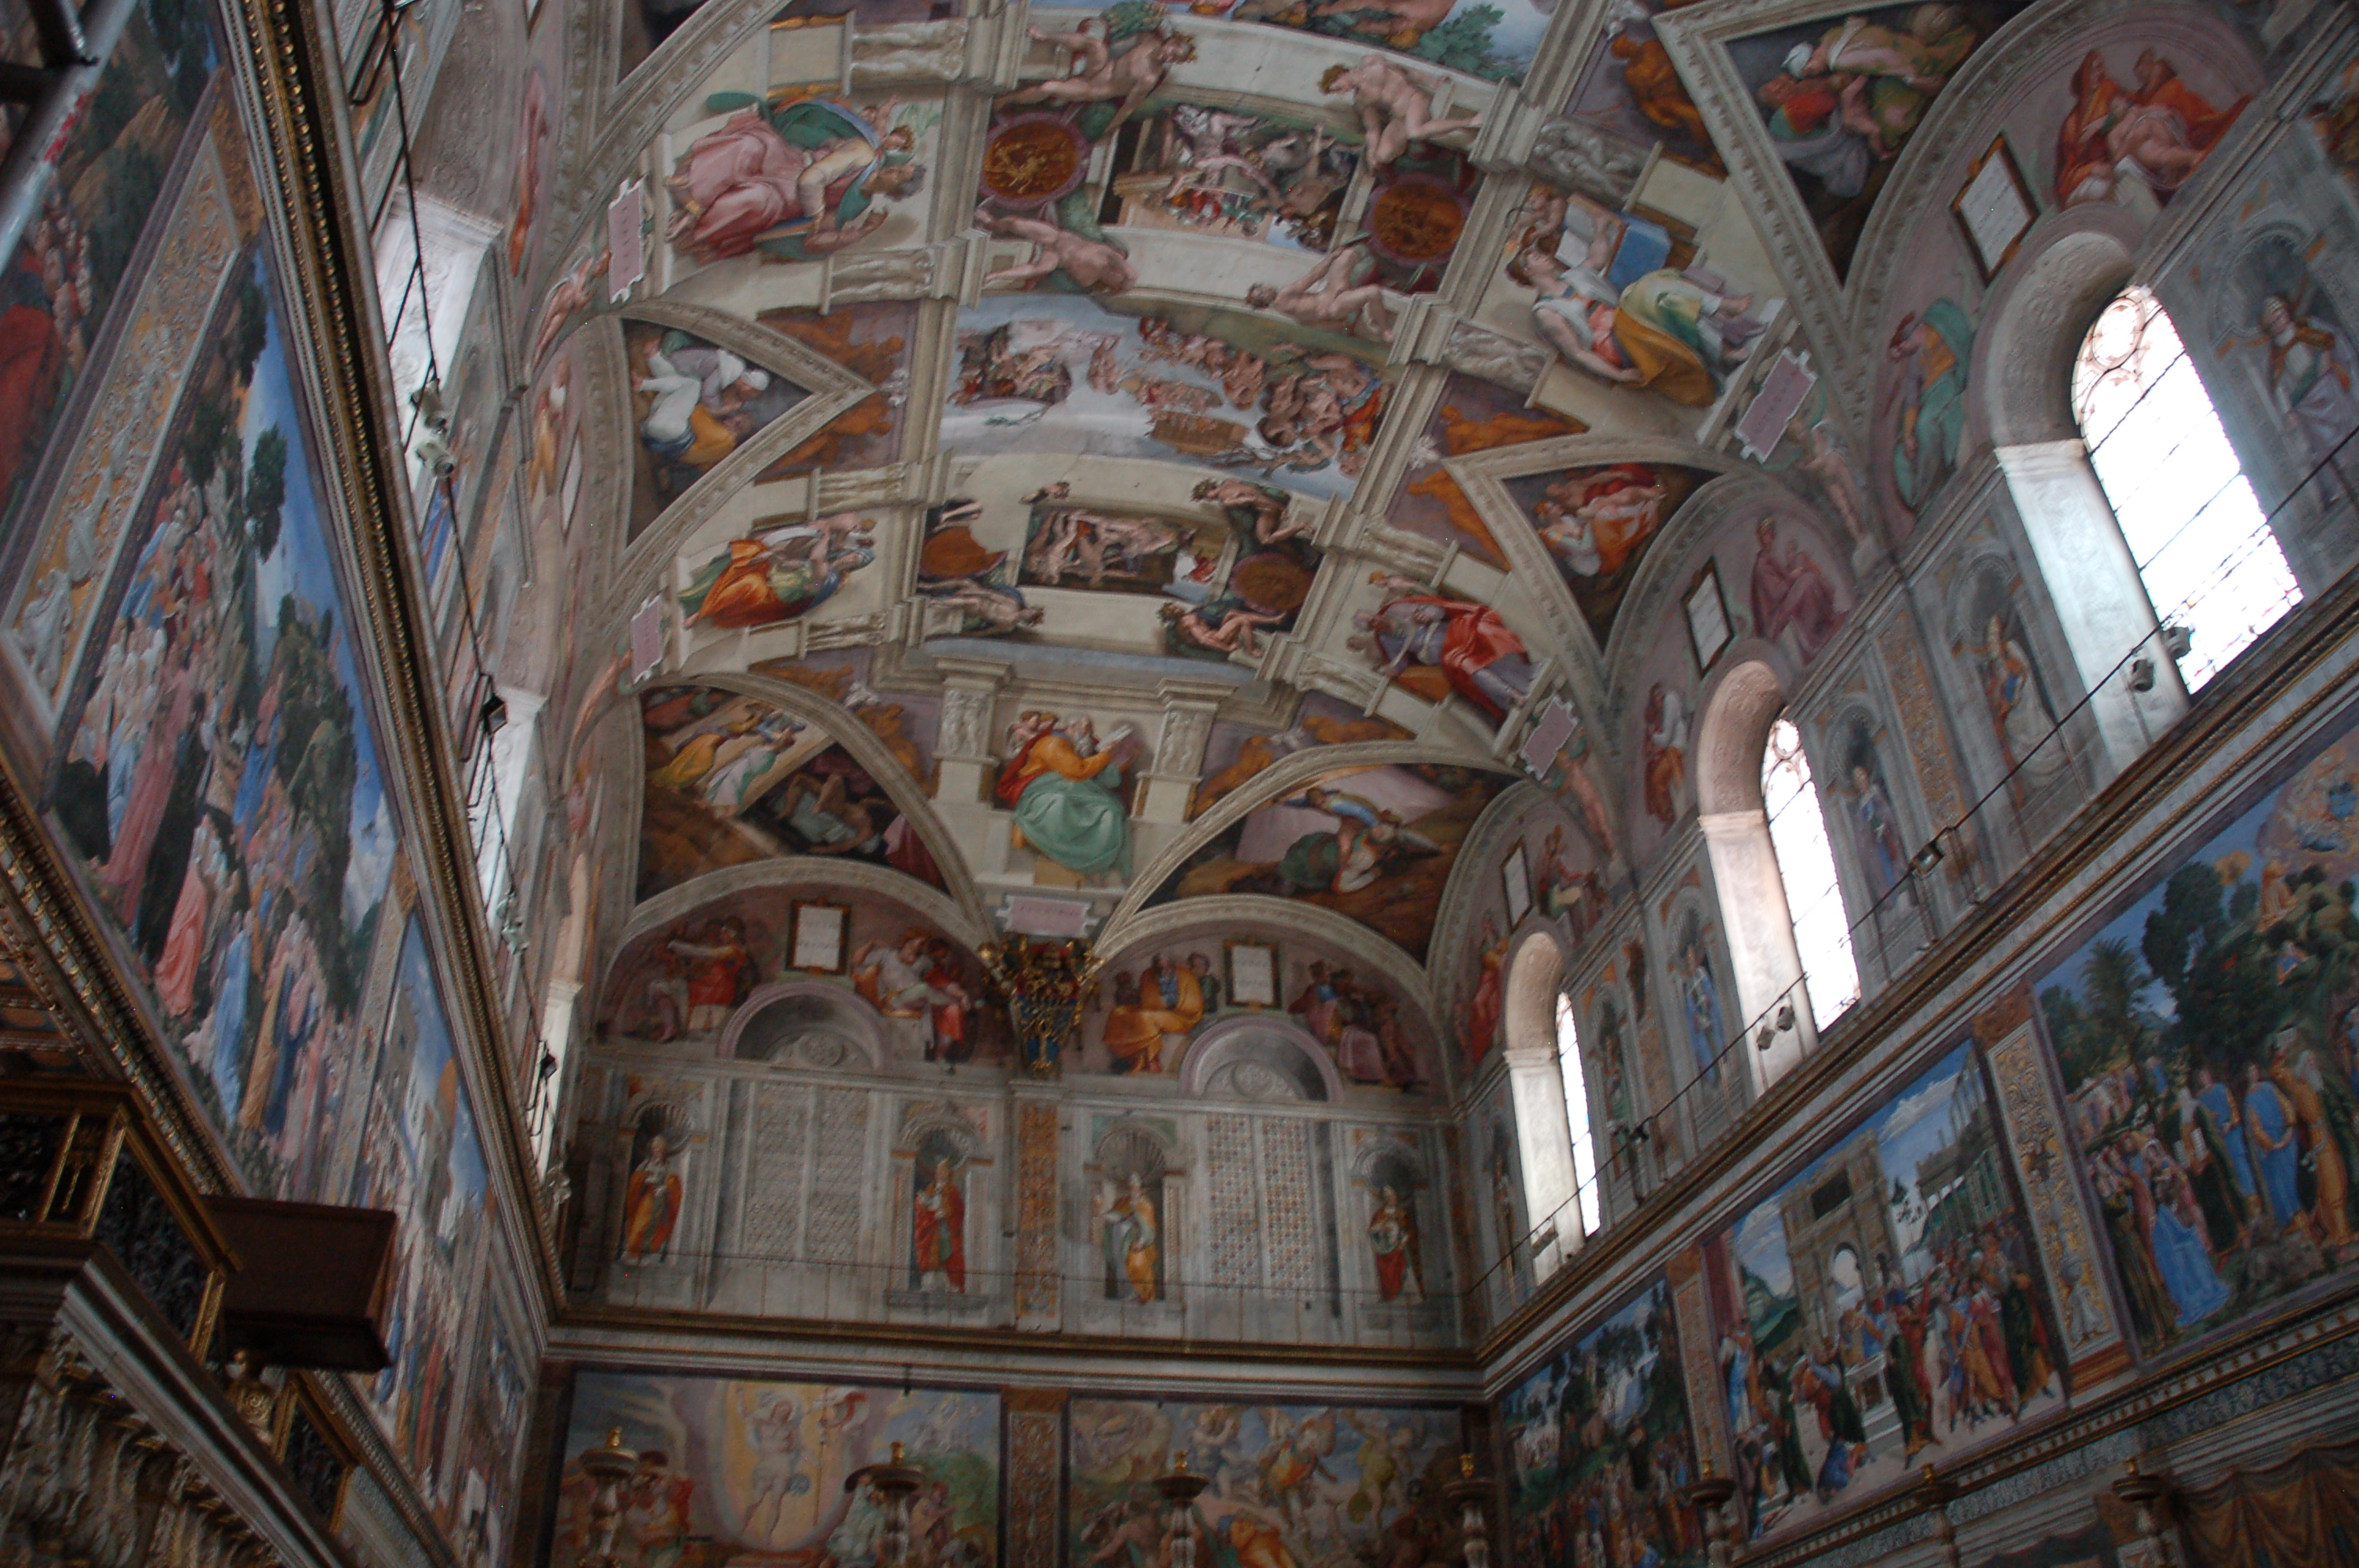
\includegraphics[width=4in]{img/img-sistine1.jpeg}
	}
	\only<8>{
		Michelangelo's \emph{Sistine Chapel} [1508--1512]
		\begin{center}
			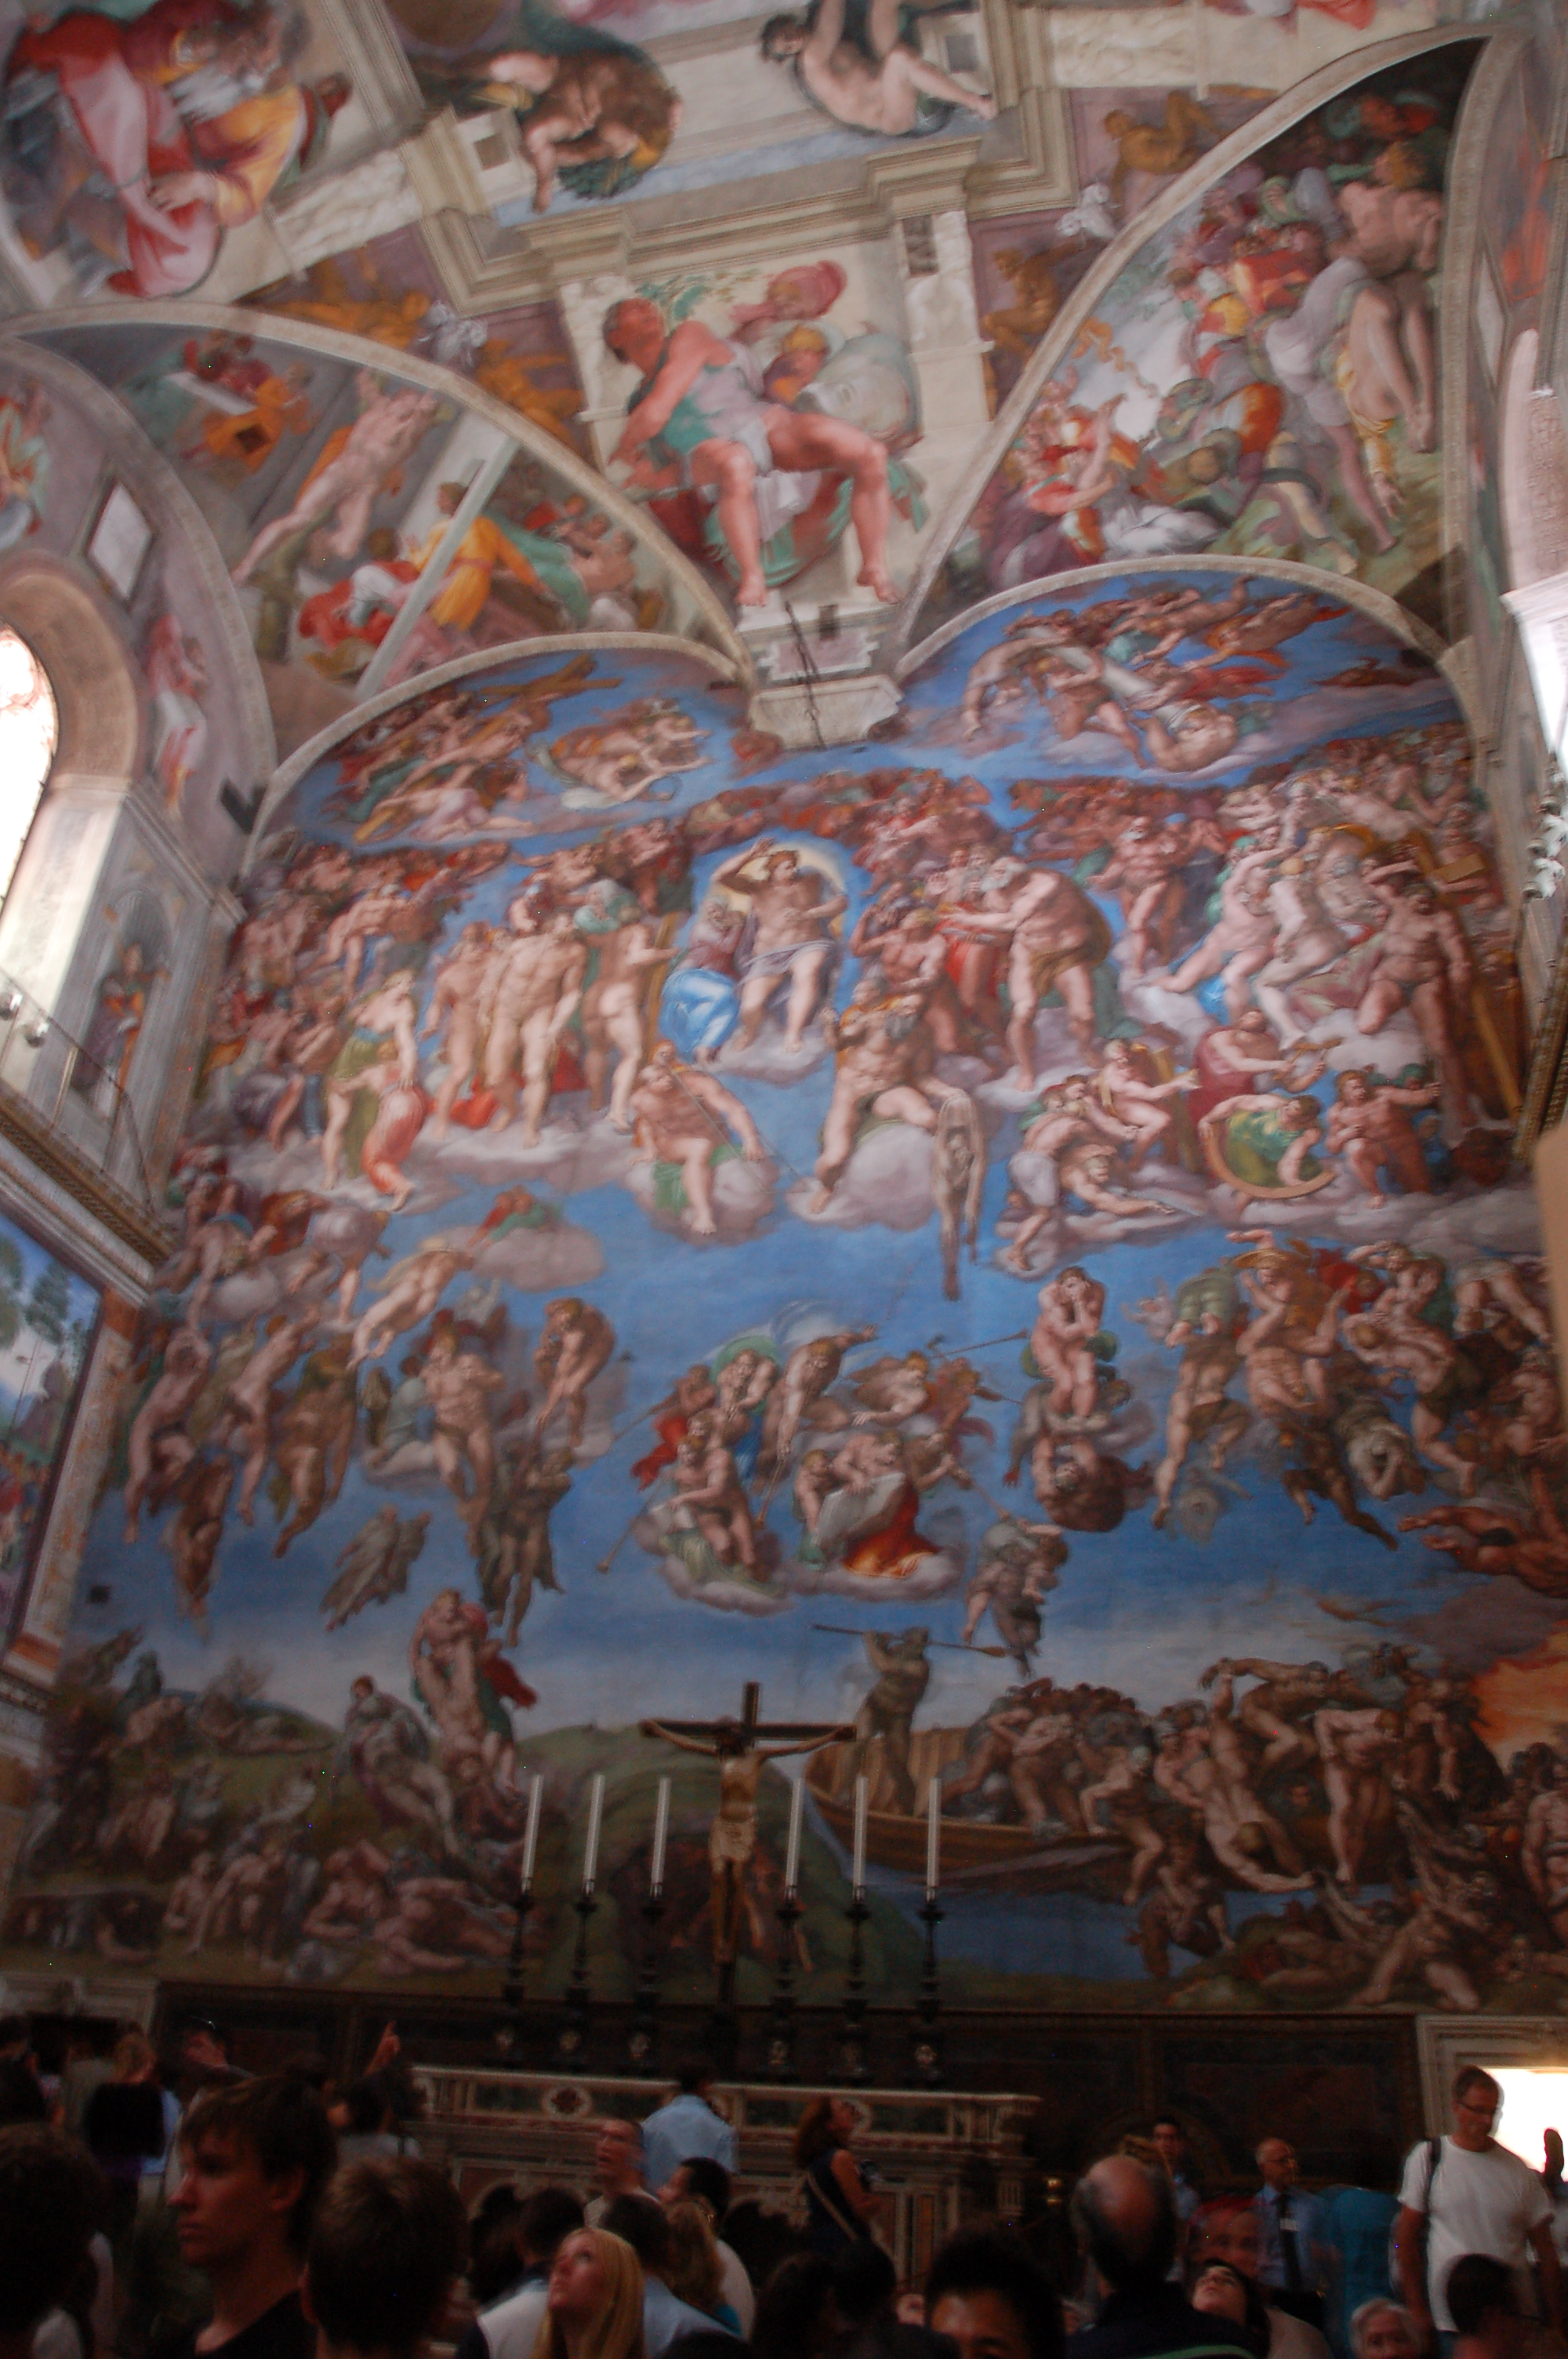
\includegraphics[height=2.8in]{img/img-sistine2.jpeg}
		\end{center}

	}
	\only<9>{
		Michelangelo's \emph{Sistine Chapel} [1508--1512]
		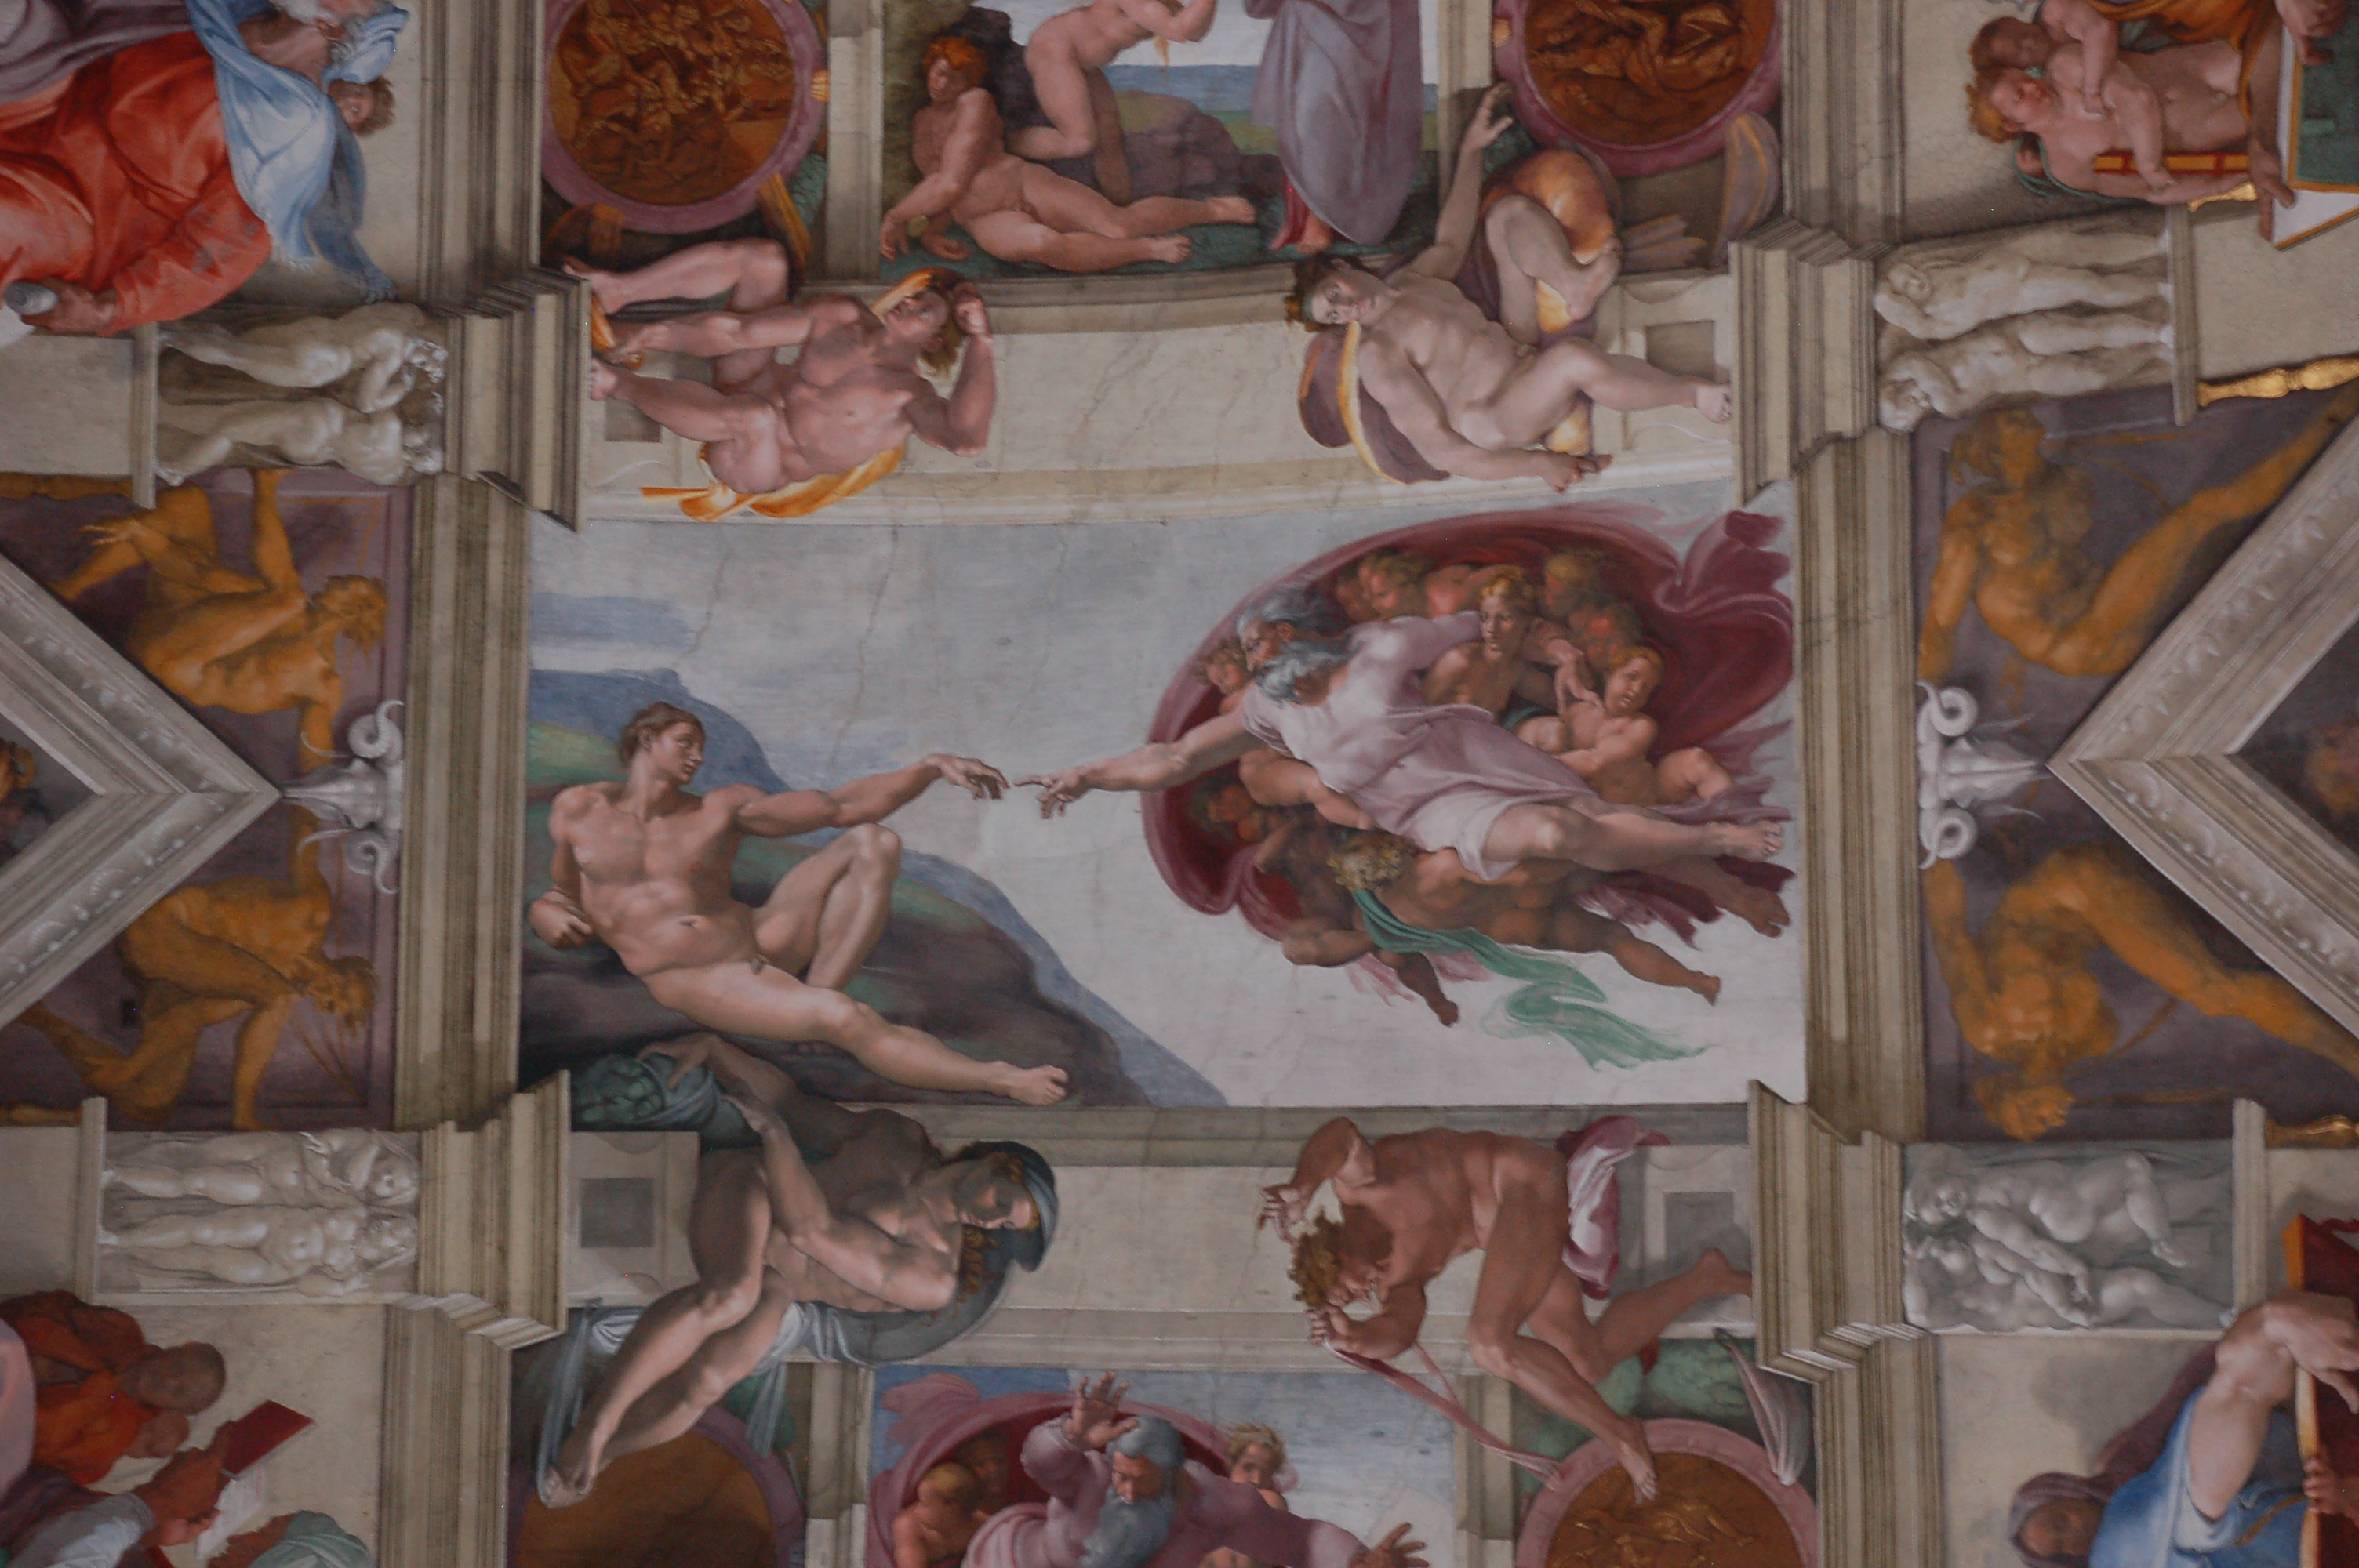
\includegraphics[width=4in]{img/img-sistine3.jpeg}
	}
	\only<10>{
		St. Peter's Basilica (Maderno, 1607--1612).
		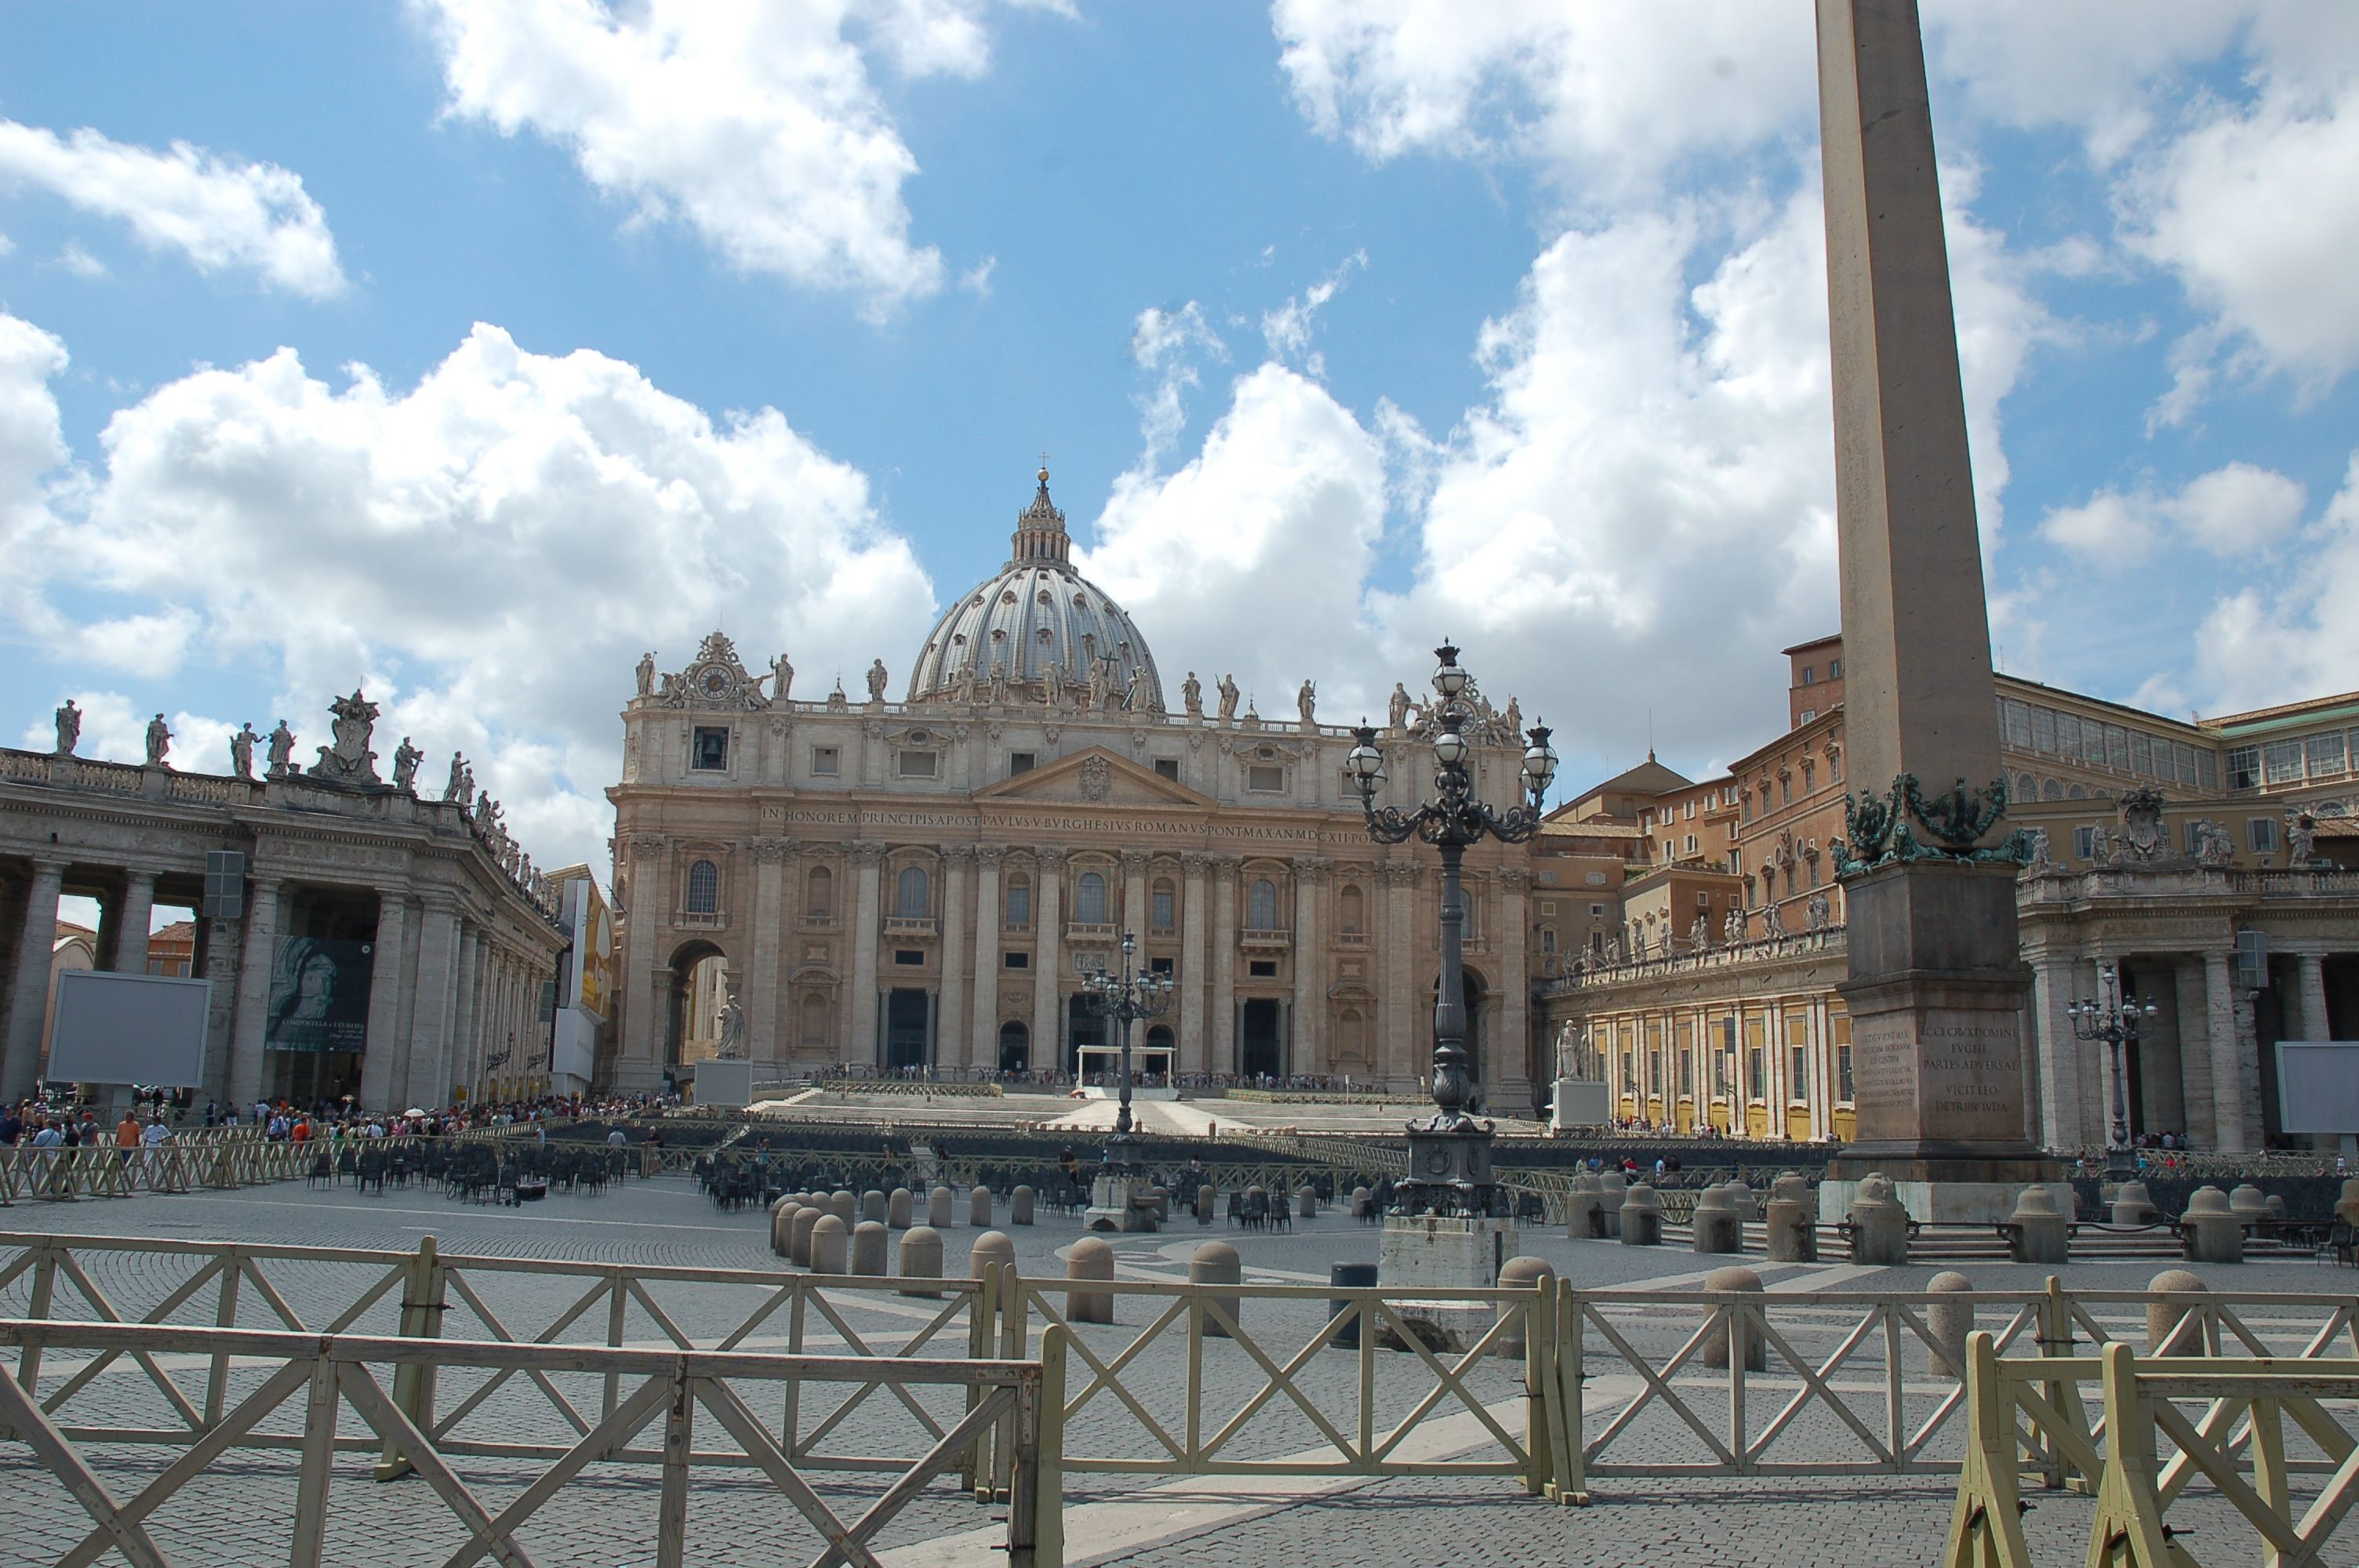
\includegraphics[width=4in]{img/img-vatican1.jpeg}
	}
	\only<11>{
		St. Peter's Basilica (Maderno, 1607--1612).
		\begin{center}
			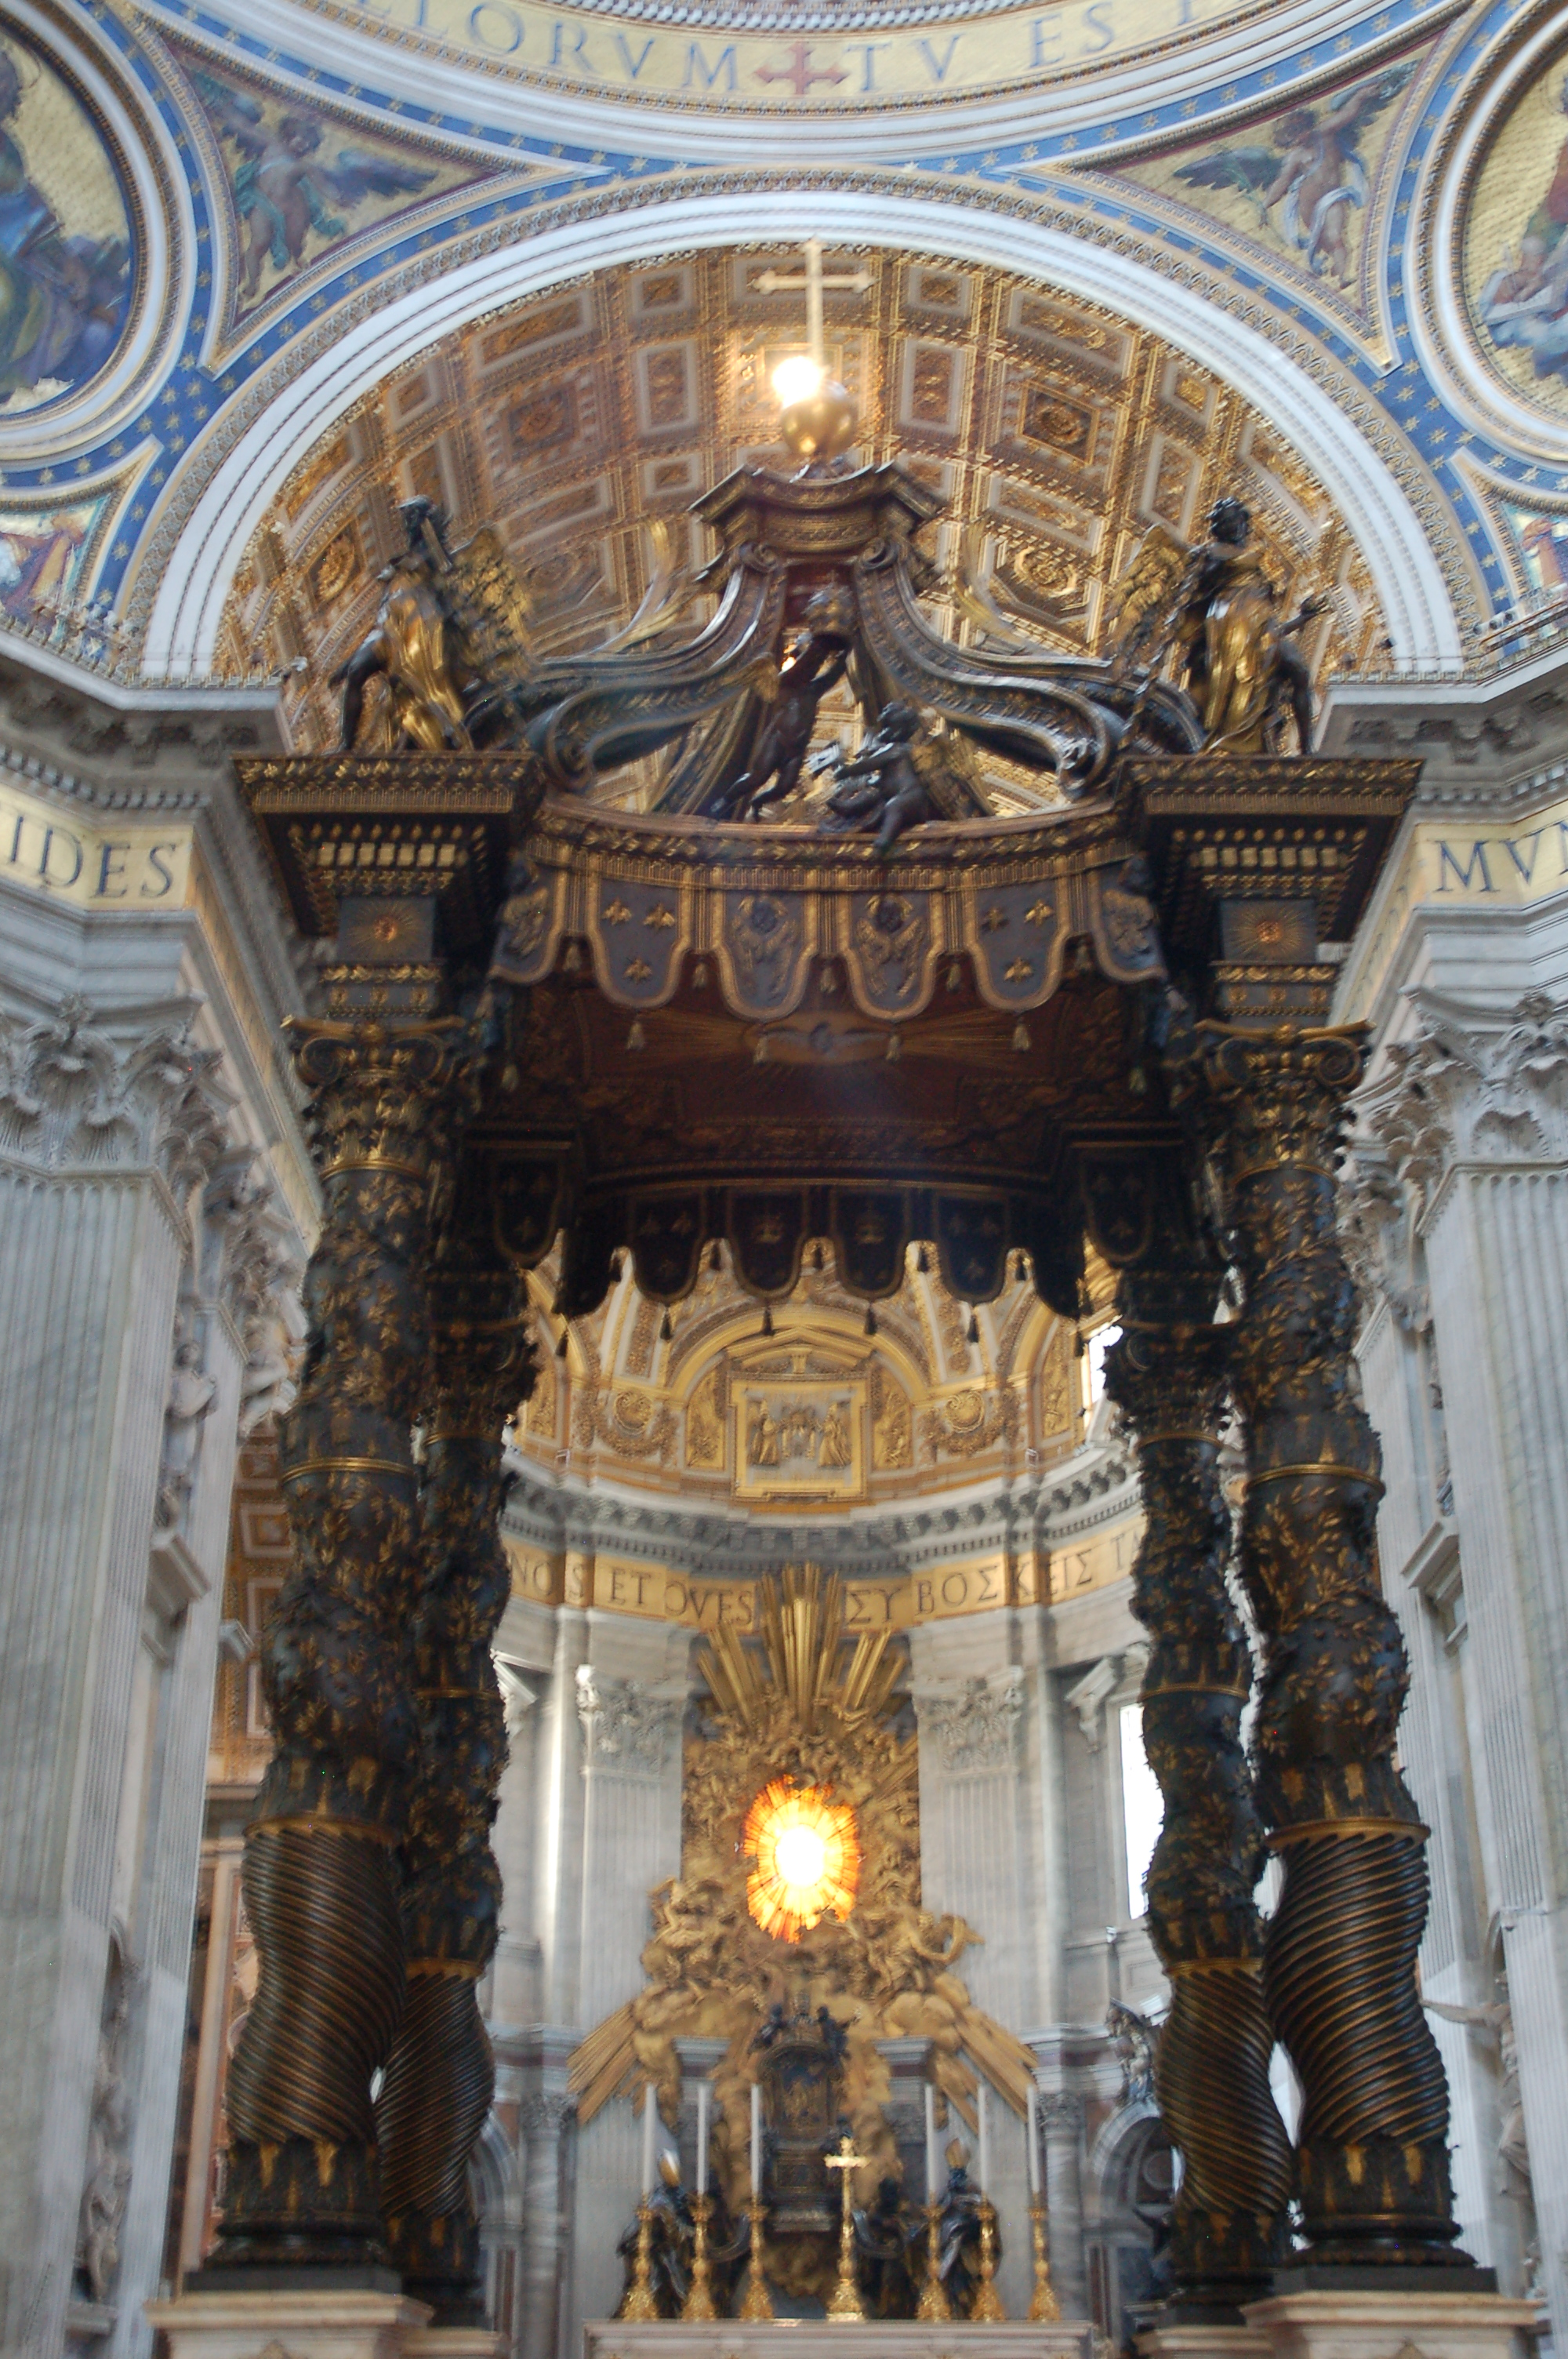
\includegraphics[height=2.8in]{img/img-vatican2.jpeg}
		\end{center}

	}
	\only<12>{
		St. Peter's Basilica (Maderno, 1607--1612).
		\begin{center}
			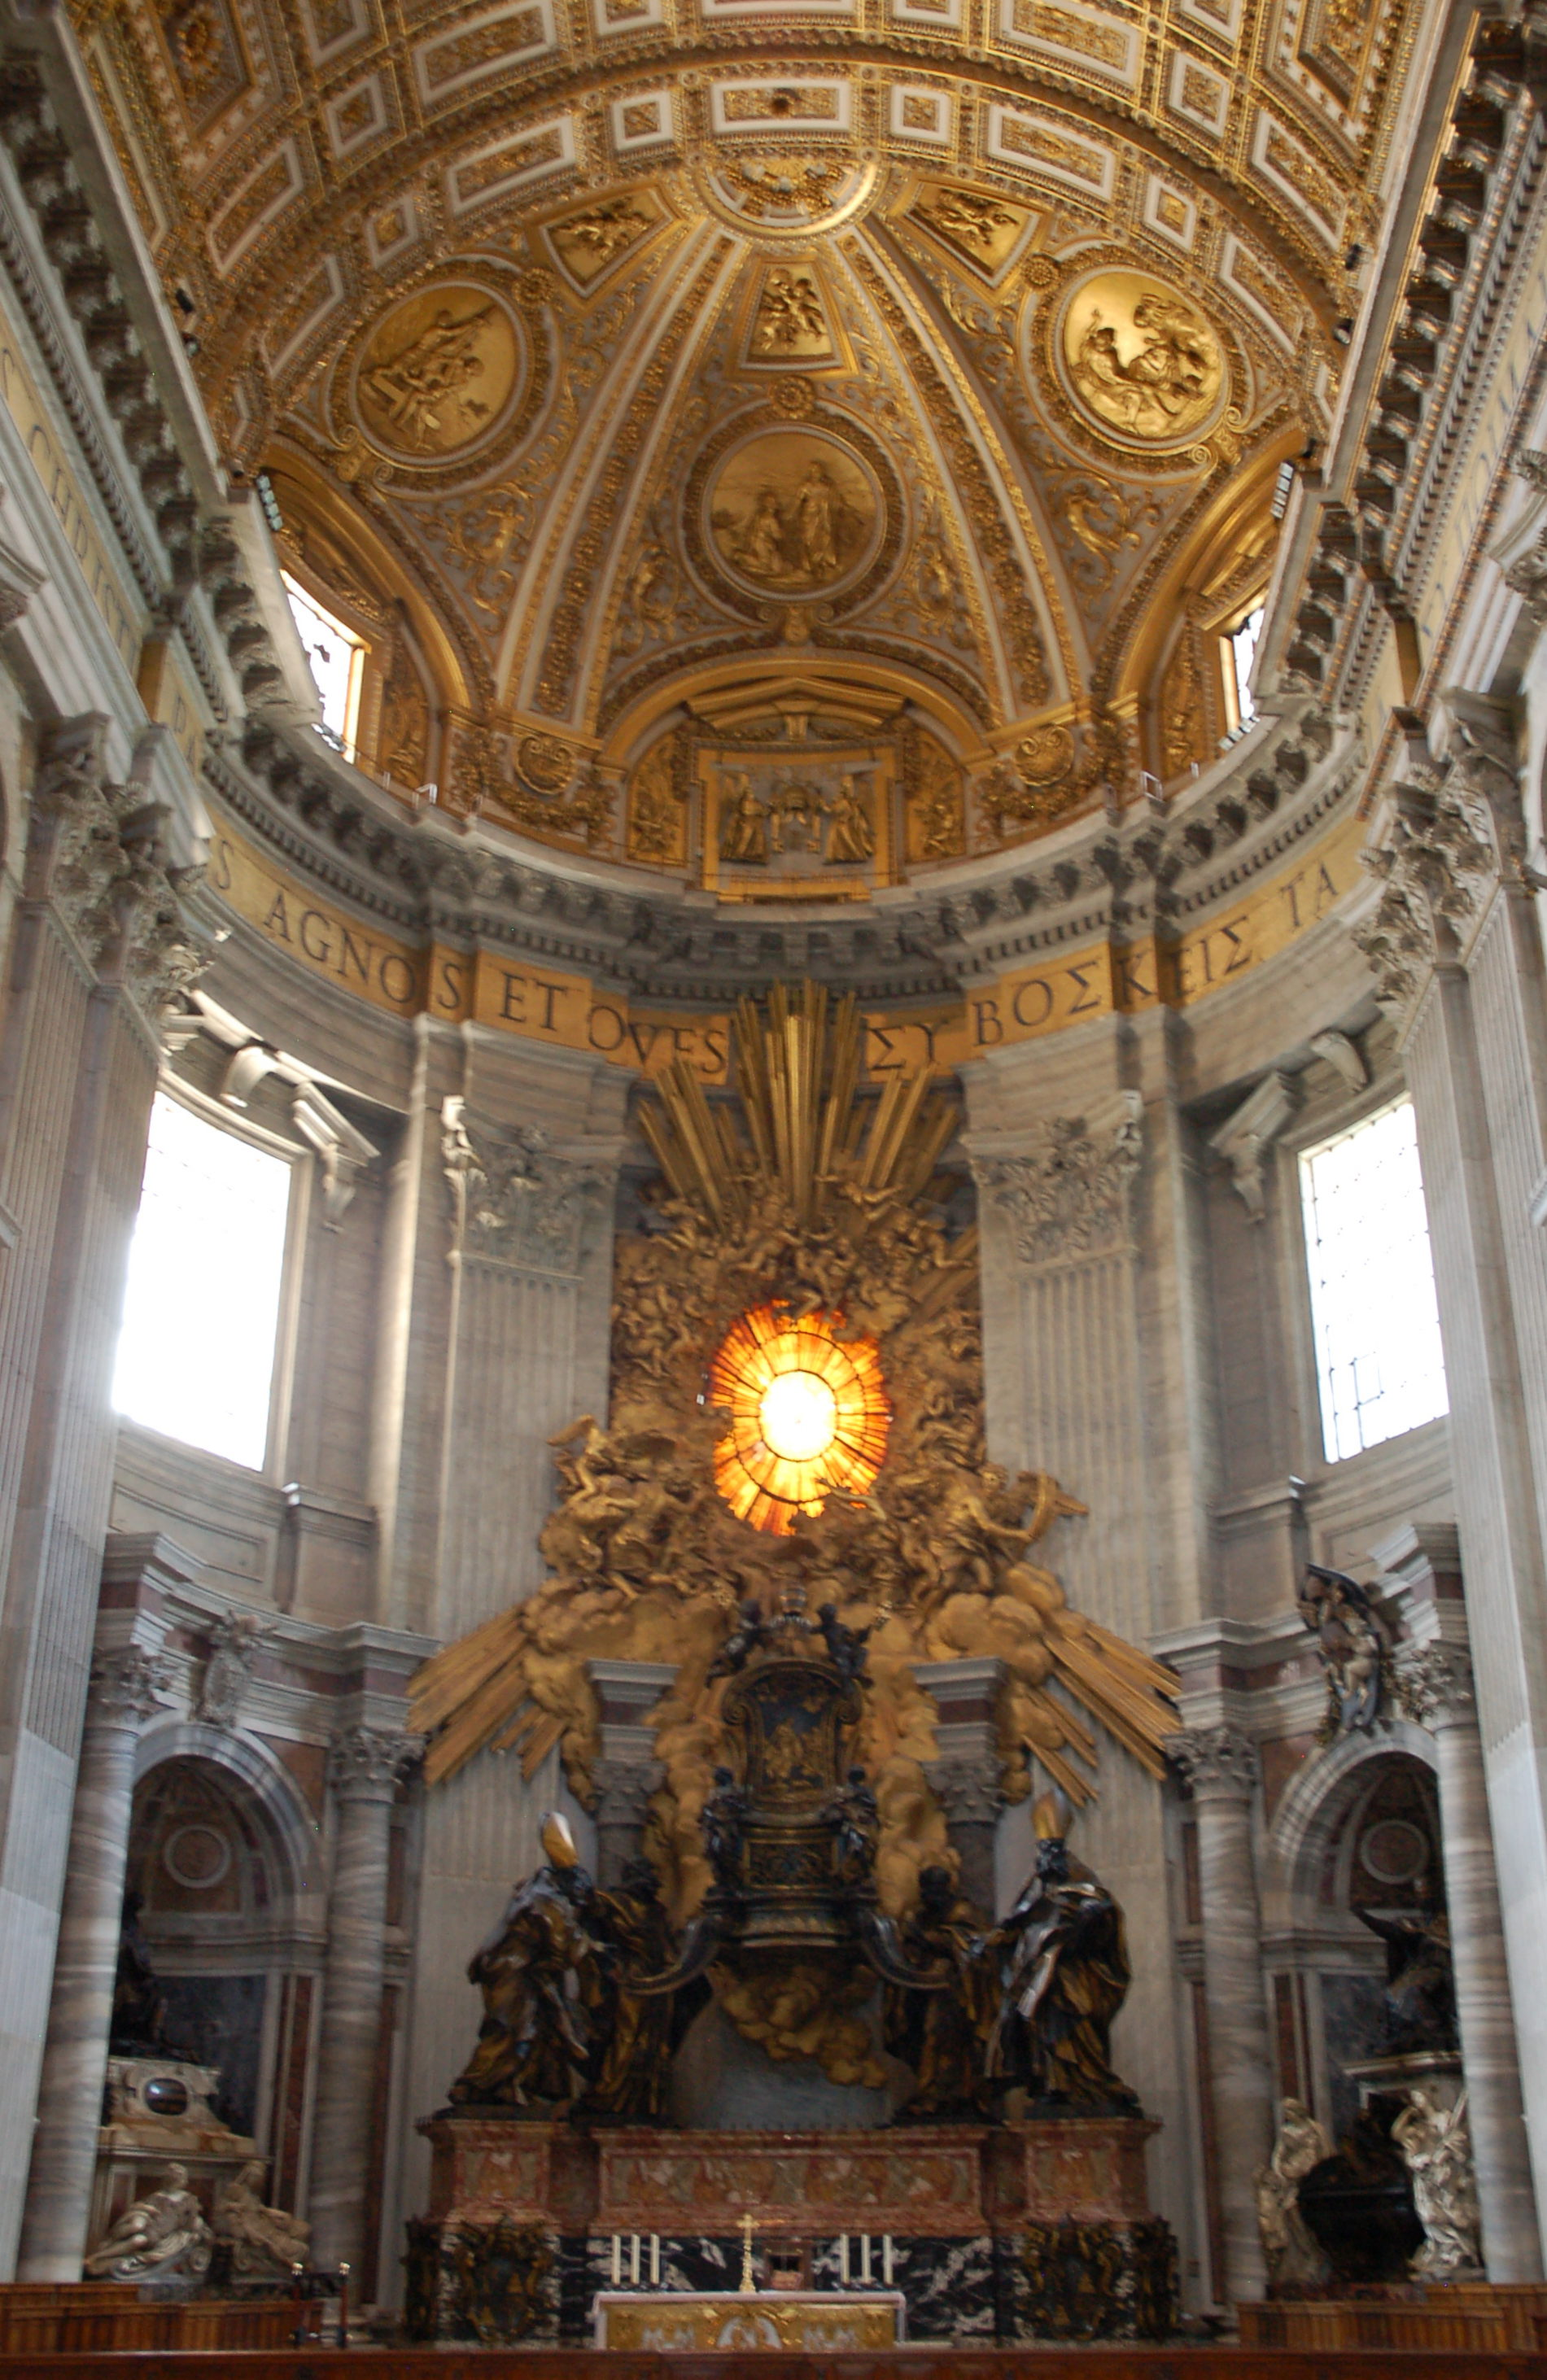
\includegraphics[height=2.8in]{img/img-vatican3.jpeg}
		\end{center}

	}
	\only<13>{
		Caravaggio's \emph{Supper at Emmaus} [1601].
		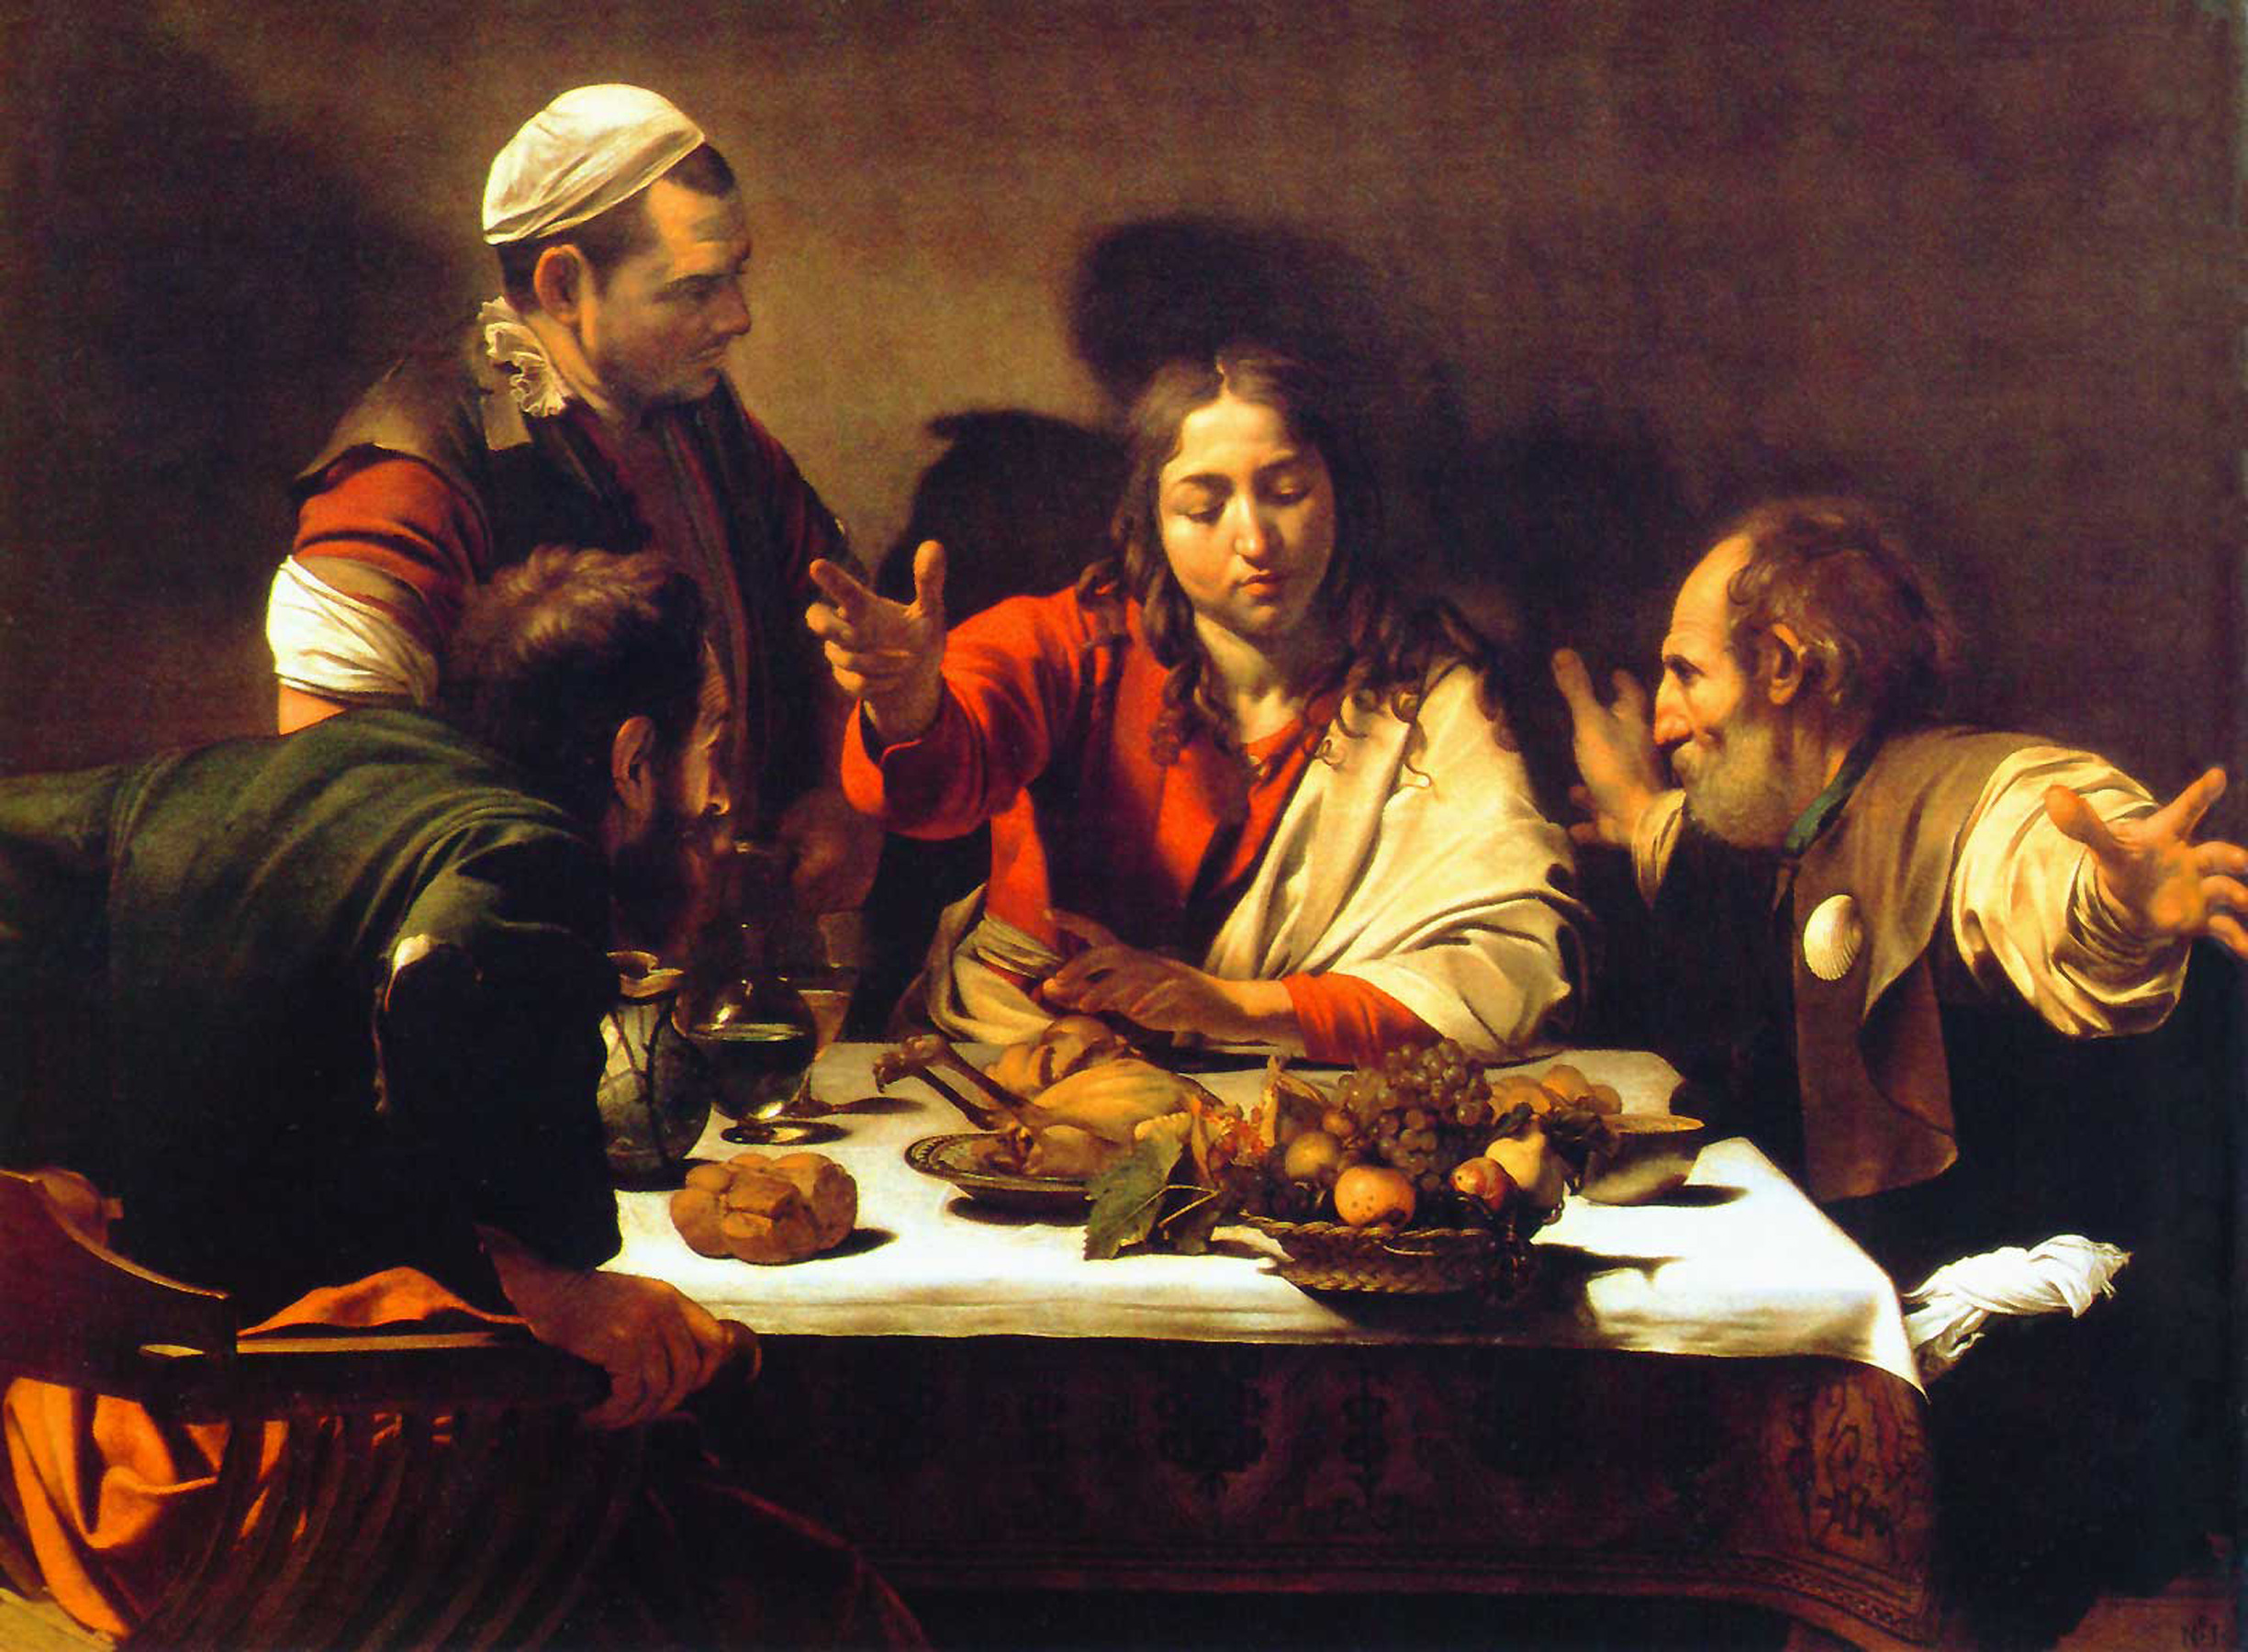
\includegraphics[width=4in]{img/img-emmaus.jpeg}
	}
\end{frame}

\subsection{Music}
\begin{frame}{Music}
	\only<1>{
		\begin{center}
			Venice \\
			\includegraphics[height=3in]{img/map-italy.pdf}
		\end{center}
	}
	\begin{itemize}
		\item<2->Giovanni Gabrieli (1557--1612). \emph{In Ecclesiis} [1615].
		\item<3->Claudio Monteverdi (1567--1643). \emph{L'Orfeo} [1607].
		\item<4->Antonio Vivaldi [1678--1741]. \emph{Four Seasons} [1723].
	\end{itemize}
\end{frame}

\section{The Northern Baroque}
\subsection{New Geography}
\begin{frame}{New Geography}
	\begin{itemize}
		\item<1-4>1560: Scottish Reformation (Mary, Queen of Scots).
		\item<2-4>1572: St. Bartholomew's Day massacre (Aug. 24 -- Oct. 3).
		\item<3-4>1581--1609: Dutch Independence (and Reformation).
		\item<4-4>1603: Union of Crowns (James VI and I).
	\end{itemize}
	\only<5>{
		\includegraphics[width=3.2in]{img/flag-scotland.png}
	}
	\only<6>{
		\includegraphics[width=3.2in]{img/flag-england.png}
	}
	\only<7>{
		\includegraphics[width=3.2in]{img/flag-gb.png}
	}
	\only<8>{
		\includegraphics[width=3.2in]{img/flag-ireland.png}
	}
	\only<9>{
		\includegraphics[width=3.2in]{img/flag-uk.png}
	}
	\begin{itemize}
		\item<10->1560: Scottish Reformation (Mary, Queen of Scots).
		\item<10->1572: St. Bartholomew's Day massacre (Aug. 24 -- Oct. 3).
		\item<10->1581--1609: Dutch Independence (and Reformation).
		\item<10->1603: Union of Crowns (James VI and I).
		\item<10->1607: Virginia colony founded.
		\item<11->1620: Puritans flee England and start new colony in modern-day Mass.
		\item<12->1648: Peace of Westphalia ends Thirty Years' War (\emph{cuius regio, eius religio}).
		\item<13->1649: Execution of King Charles I. Reign of PM Cromwell.
	\end{itemize}
\end{frame}

\subsection{"Secular" Art}
\begin{frame}{"Secular" Art}
	\only<1>{
		Johannes Vermeer's \emph{The Geographer} [1668--1669].
		\begin{center}
			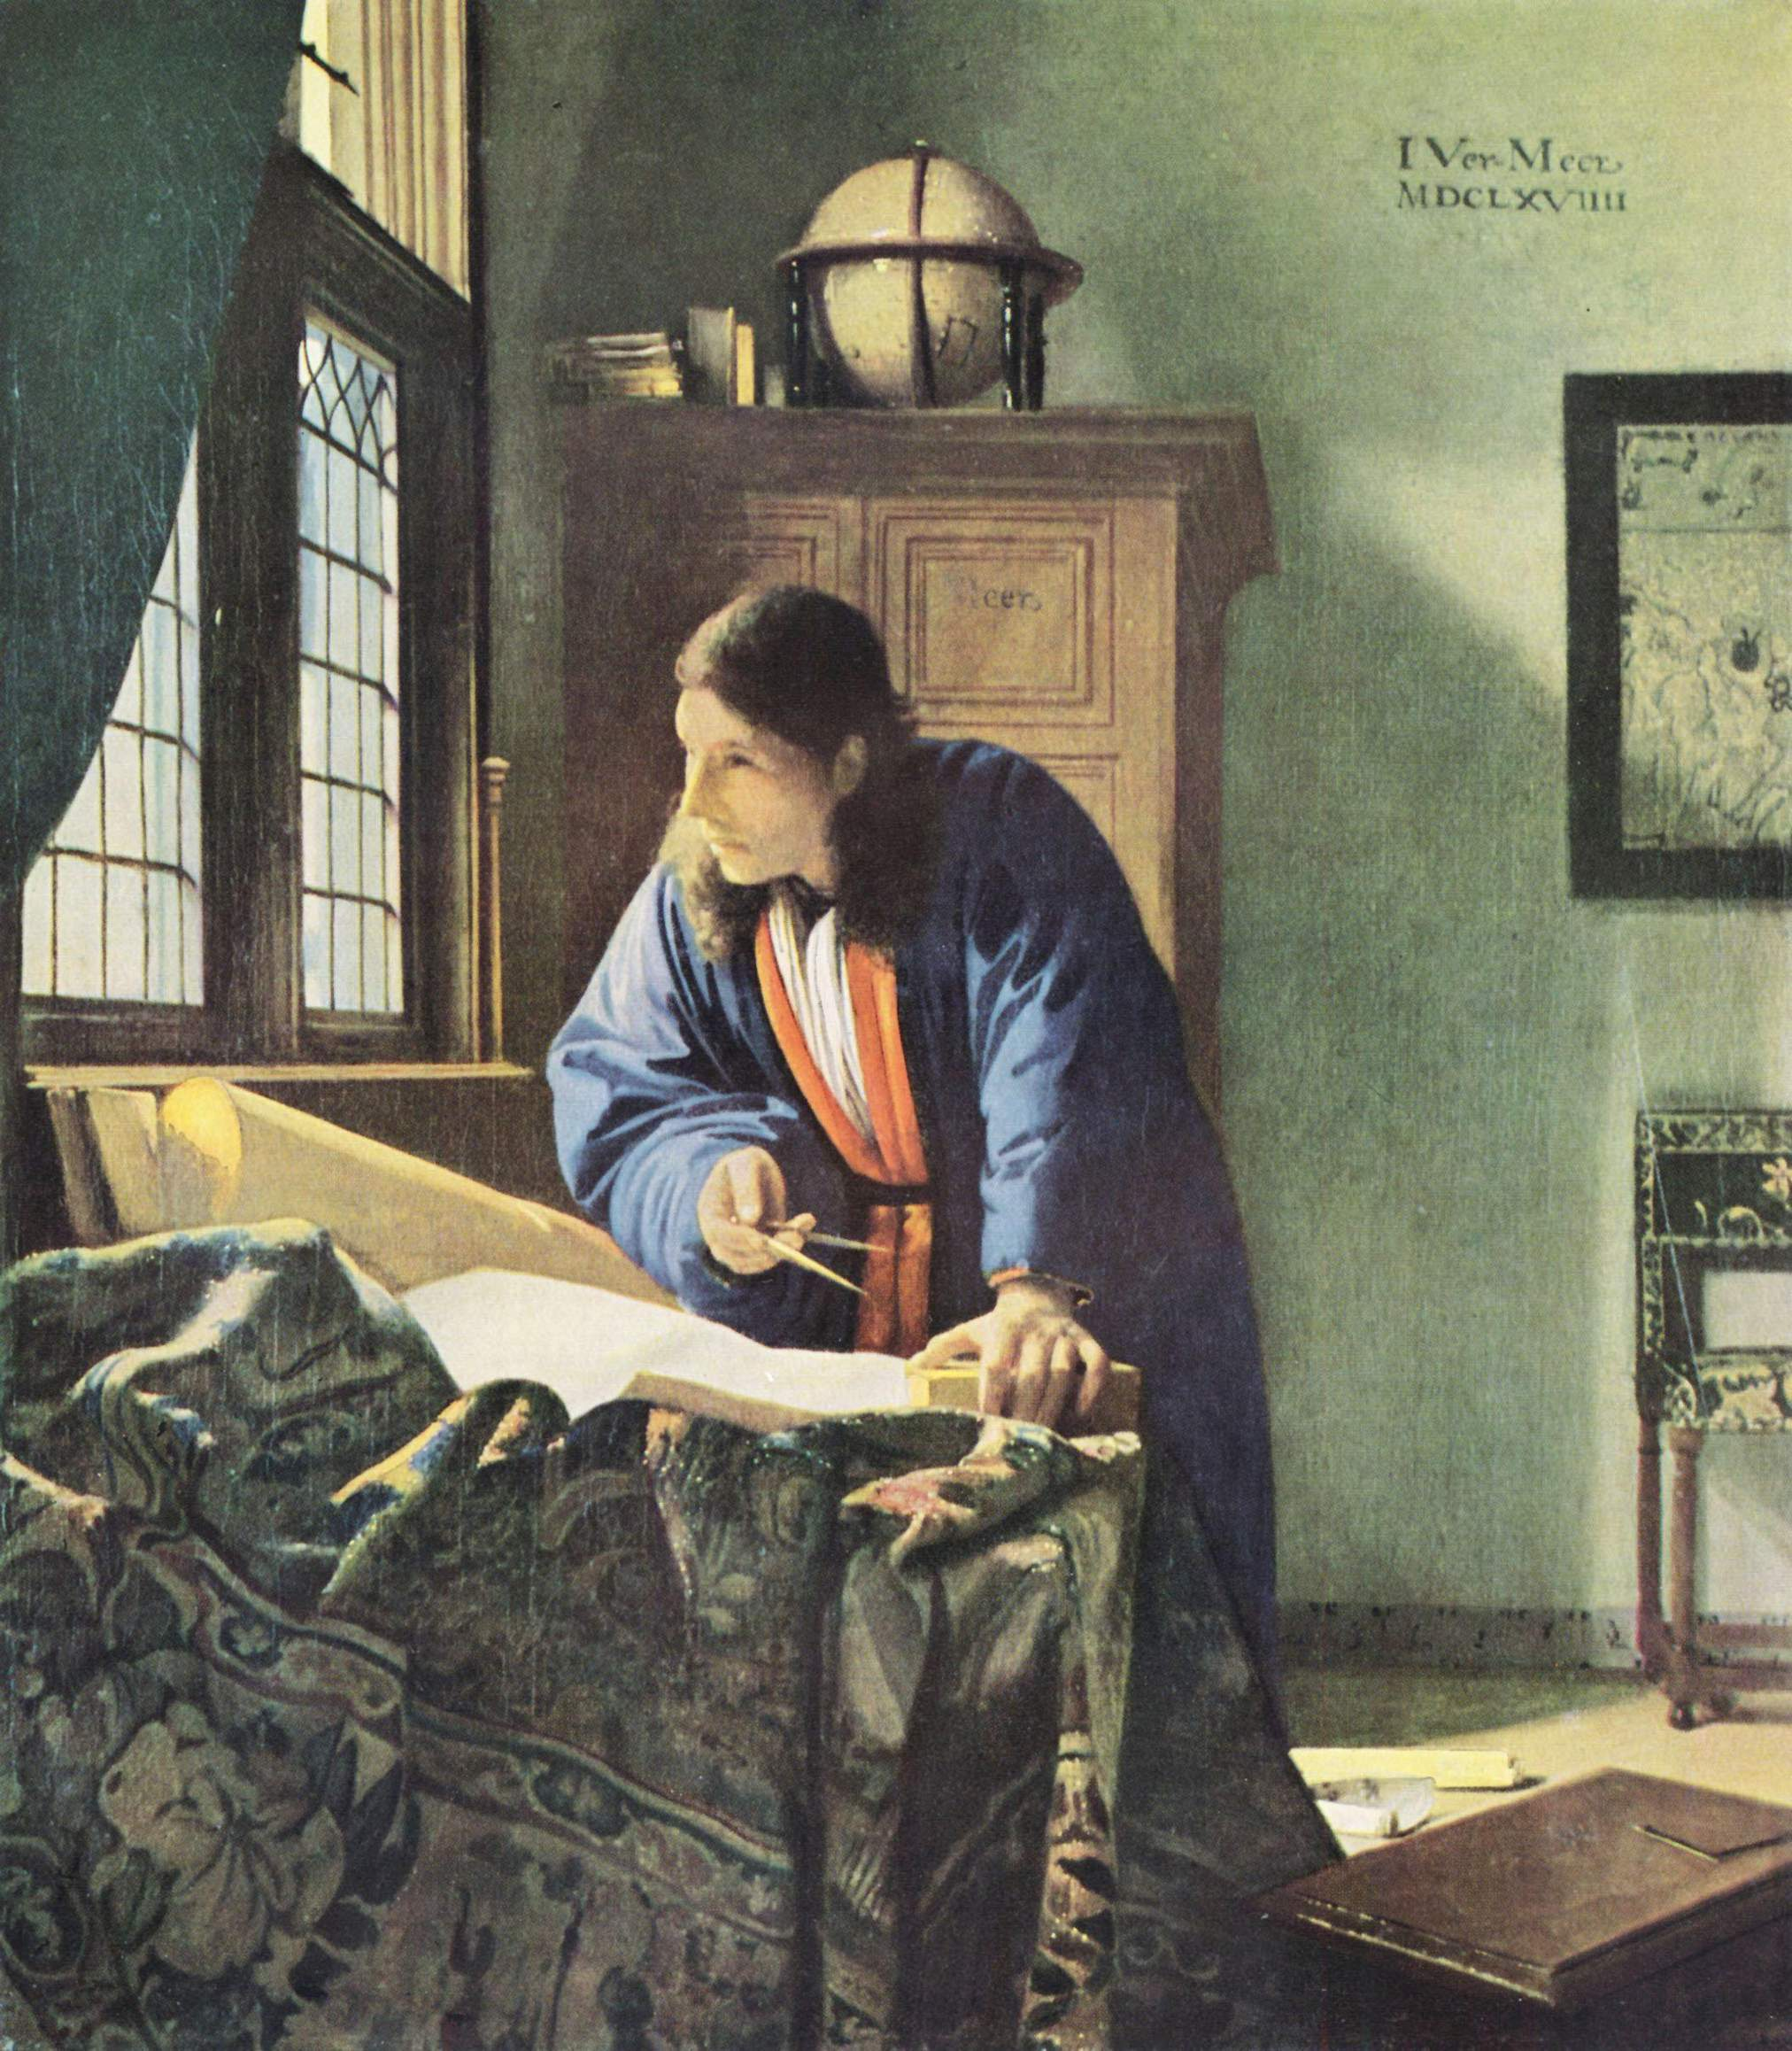
\includegraphics[height=2.9in]{img/img-geographer.jpeg}
		\end{center}

	}
	\only<2>{
	Rembrandt's \emph{The Anatomy Lesson of Dr. Tulp} [1632]
		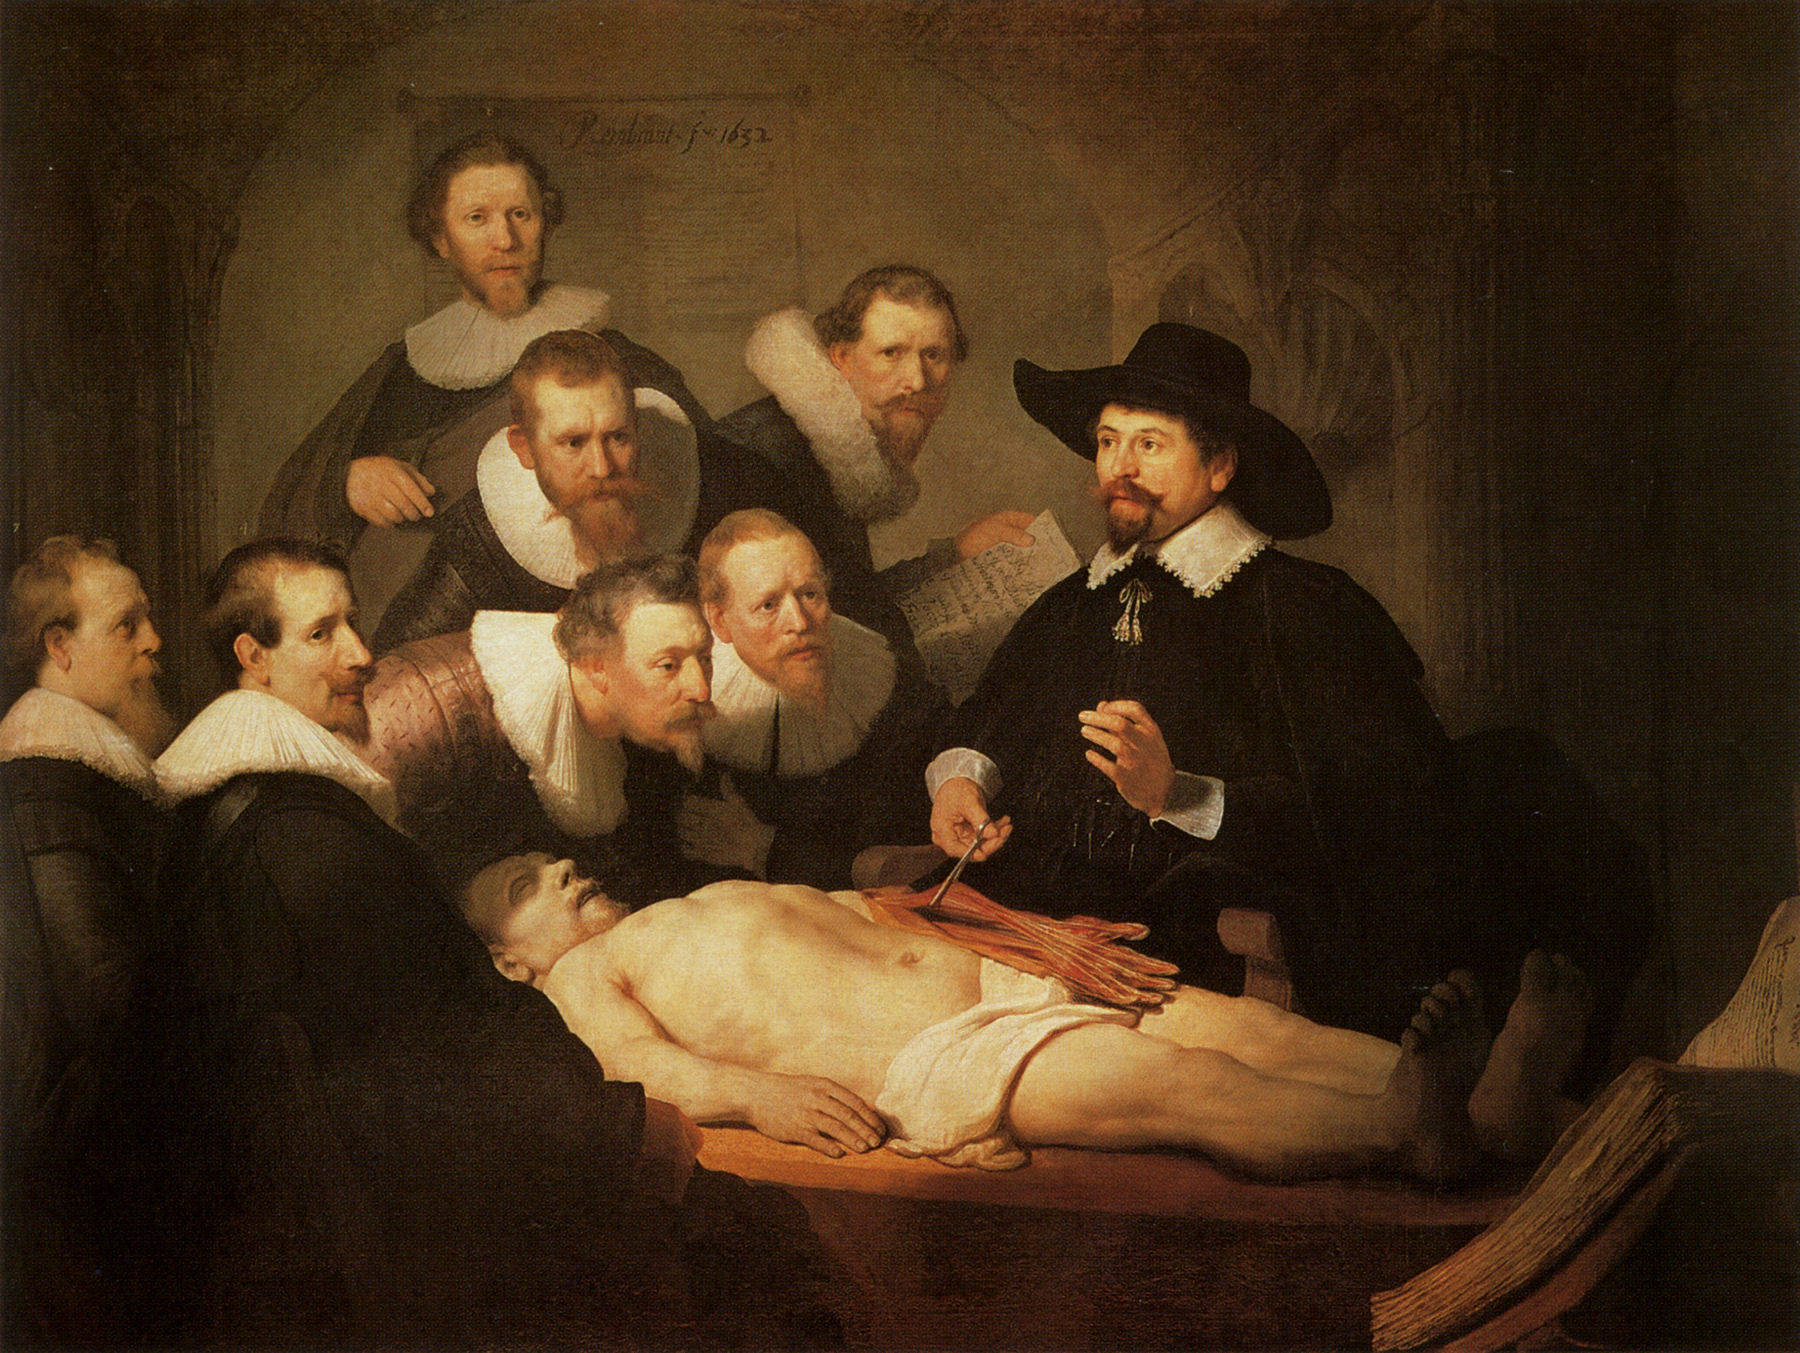
\includegraphics[width=4in]{img/img-tulp.jpeg}
	}
\end{frame}

\subsection{Towards Enlightenment}
\begin{frame}{New Methods}
	\begin{itemize}
		\item<1->Francis Bacon [1561--1626] (empirical method).
		\item<2->William Shakespeare [1564--1616].
		\item<3->Galileo Galilee [1564--1642].
		\item<4->Johannes Kepler (1571--1630).
		\item<5->Ren{\'e} Descartes [1596--1650] (deductive reasoning).
	\end{itemize}
\end{frame}

